\documentclass[a4paper,20pt,oneside]{book}
\usepackage[utf8]{inputenc} 
\usepackage[T1]{fontenc} 
\usepackage[nonumberlist]{glossaries} 
\usepackage[english,ngerman]{babel}
\usepackage{float}
\usepackage{graphicx}
\usepackage{longtable}
\usepackage{titlesec}
\usepackage{pdfpages}
\usepackage{glossaries}
\usepackage{listings}
\usepackage{color}
\usepackage{titlepic}
\usepackage{booktabs}
\usepackage{ulem}
\usepackage[document]{ragged2e}
\usepackage[DIV=14,BCOR=2mm,headinclude=true,footinclude=false]{typearea}
\definecolor{dkgreen}{rgb}{0,0.6,0}
\definecolor{gray}{rgb}{0.5,0.5,0.5}
\definecolor{mauve}{rgb}{0.58,0,0.82}
\lstset{frame=tb,
	language=bash,
	aboveskip=3mm,
	belowskip=3mm,
	showstringspaces=false,
	columns=flexible,
	basicstyle={\small\ttfamily},
	numbers=none,
	numberstyle=\tiny\color{gray},
	keywordstyle=\color{blue},
	commentstyle=\color{dkgreen},
	stringstyle=\color{mauve},
	breaklines=true,
	breakatwhitespace=true,
	tabsize=3
}
\titleformat{\subparagraph}
{\normalfont\normalsize\bfseries}{\thesubparagraph}{1em}{}
\titlespacing*{\subparagraph}{\parindent}{3.25ex plus 1ex minus .2ex}{.75ex plus .1ex}

\makeglossaries



\begin{document}
	\title{\Huge{\bfseries{Entwurfsphase}}}
	\author{}
	\maketitle
	\clearpage
	
	\tableofcontents
	
	\chapter{Klassen}
	\section{Klassendiagramm}
	\subsection{Grobstruktur}
	    \begin{figure}[!hb]
	    	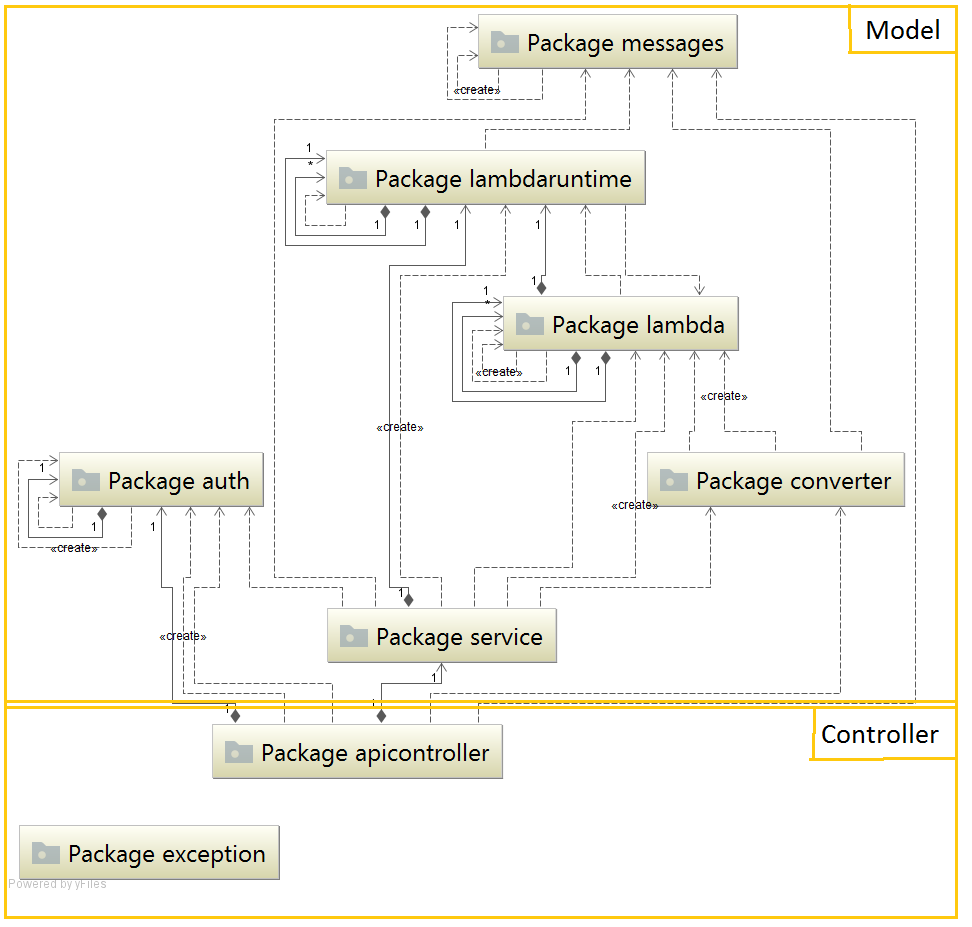
\includegraphics[width=18cm,height=13cm]{globaldiagram}
	    \end{figure}	
    \clearpage
    
    \subsection{ApiController}
	    \begin{figure}[!hb]
	    	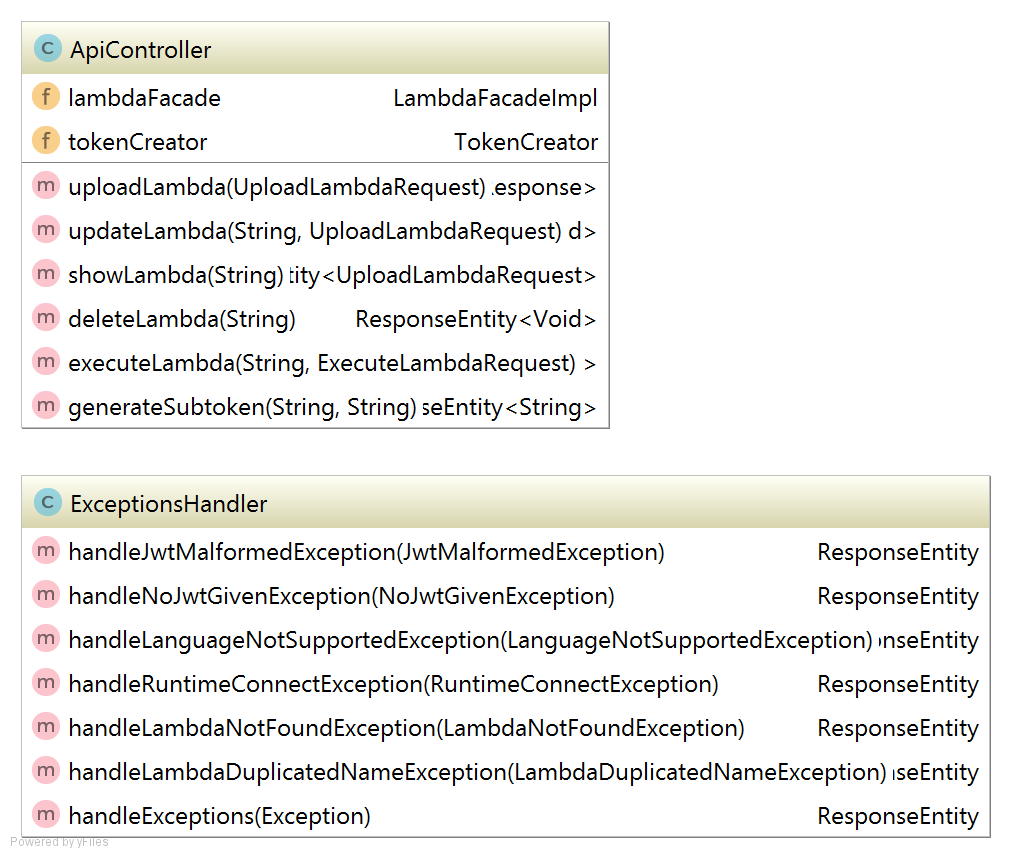
\includegraphics[width=18cm,height=20cm]{controllerdiagram}
	    \end{figure}
    \subsection{Model}
	    \begin{figure}[!hb]
	    	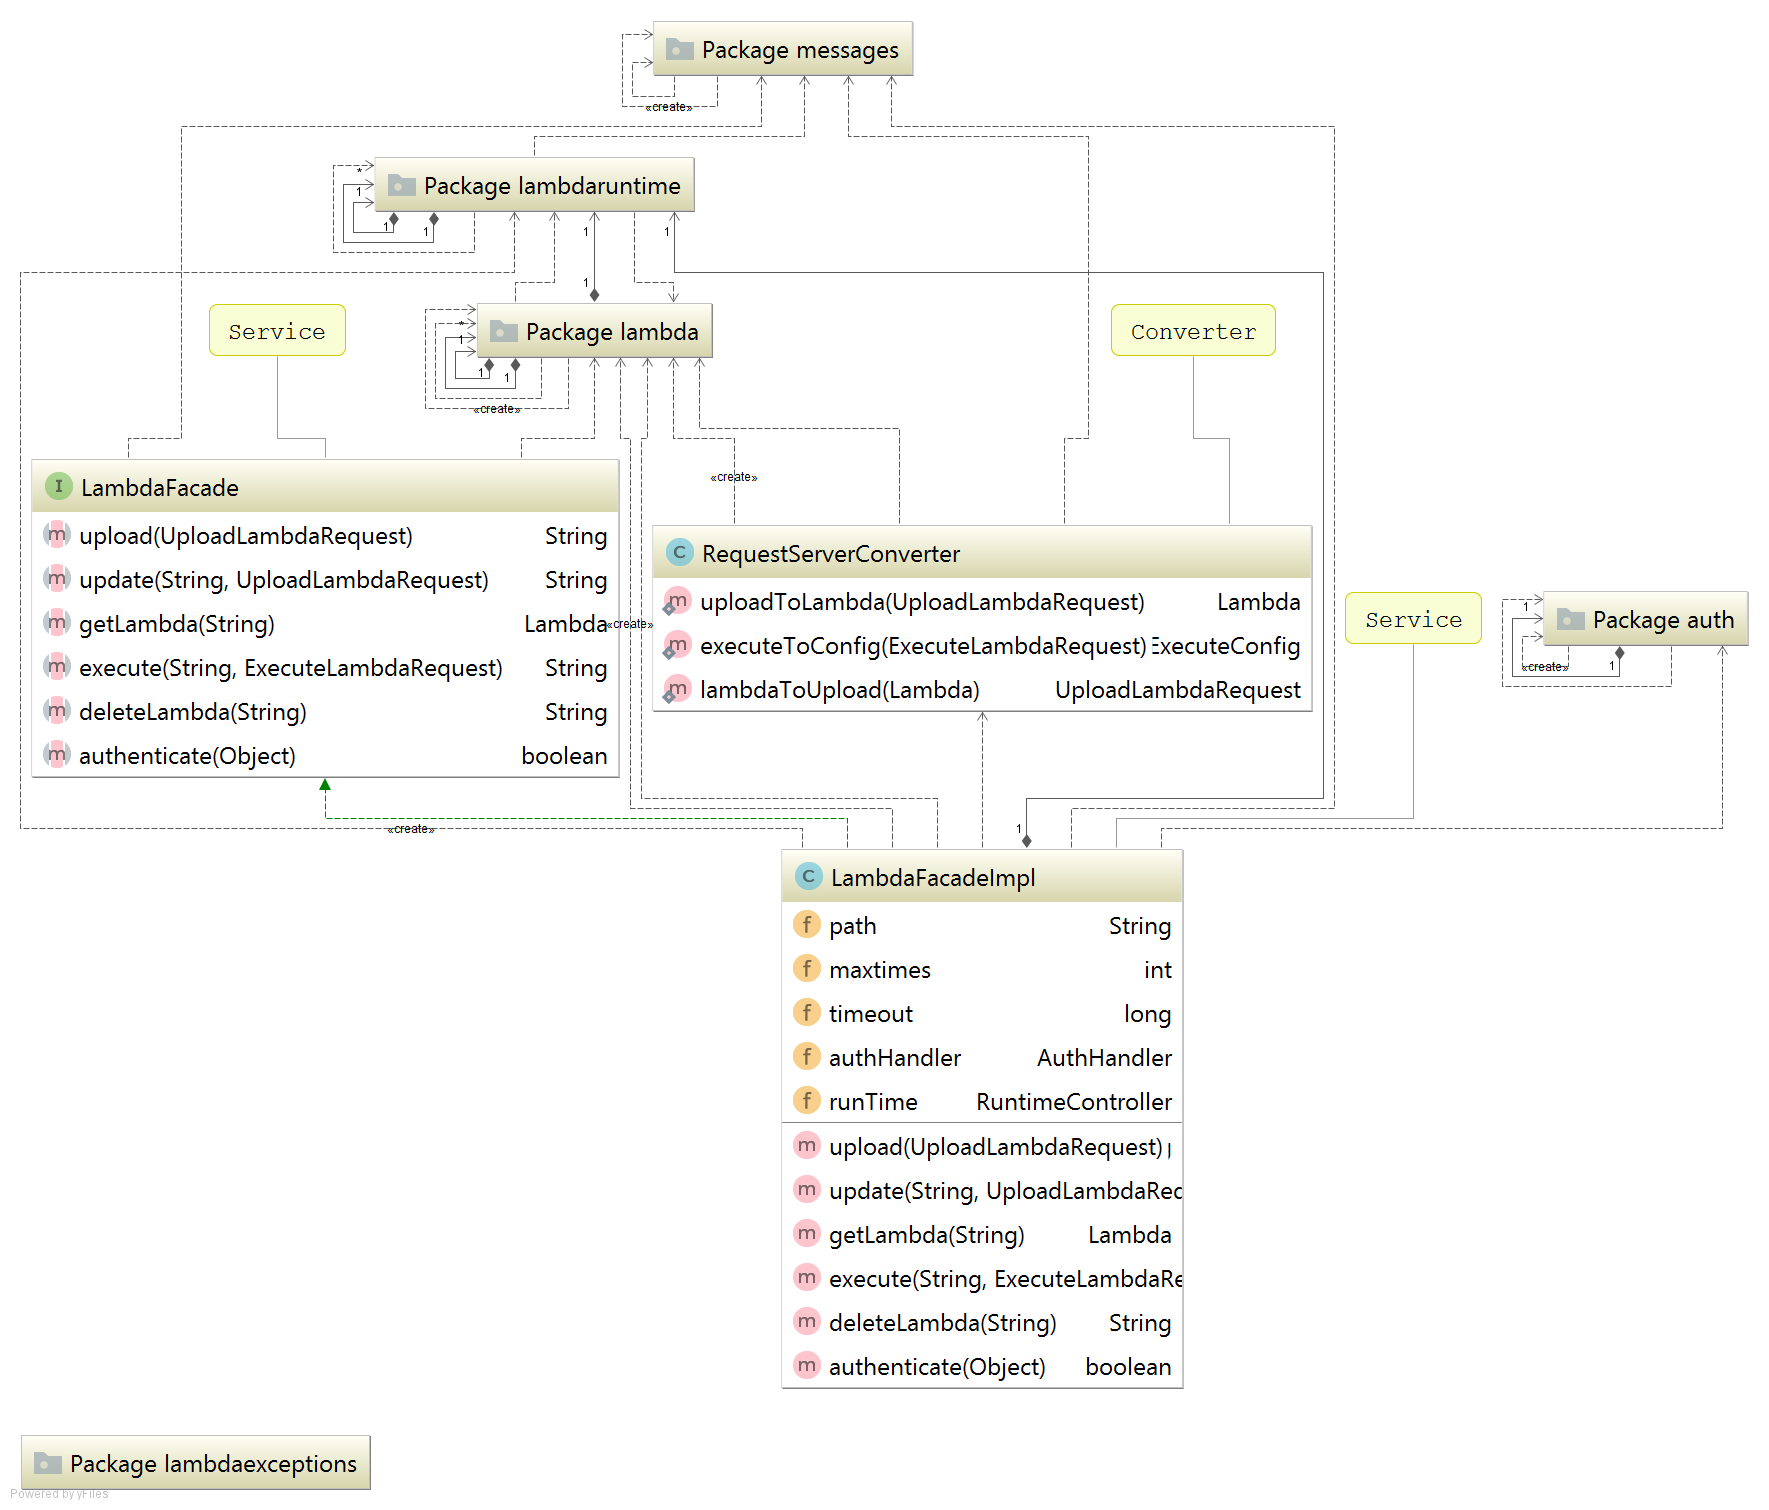
\includegraphics[width=18cm,height=20cm]{modeldiagram}
	    \end{figure}
    \subsection{Lambda}
	    \begin{figure}[!hb]
	    	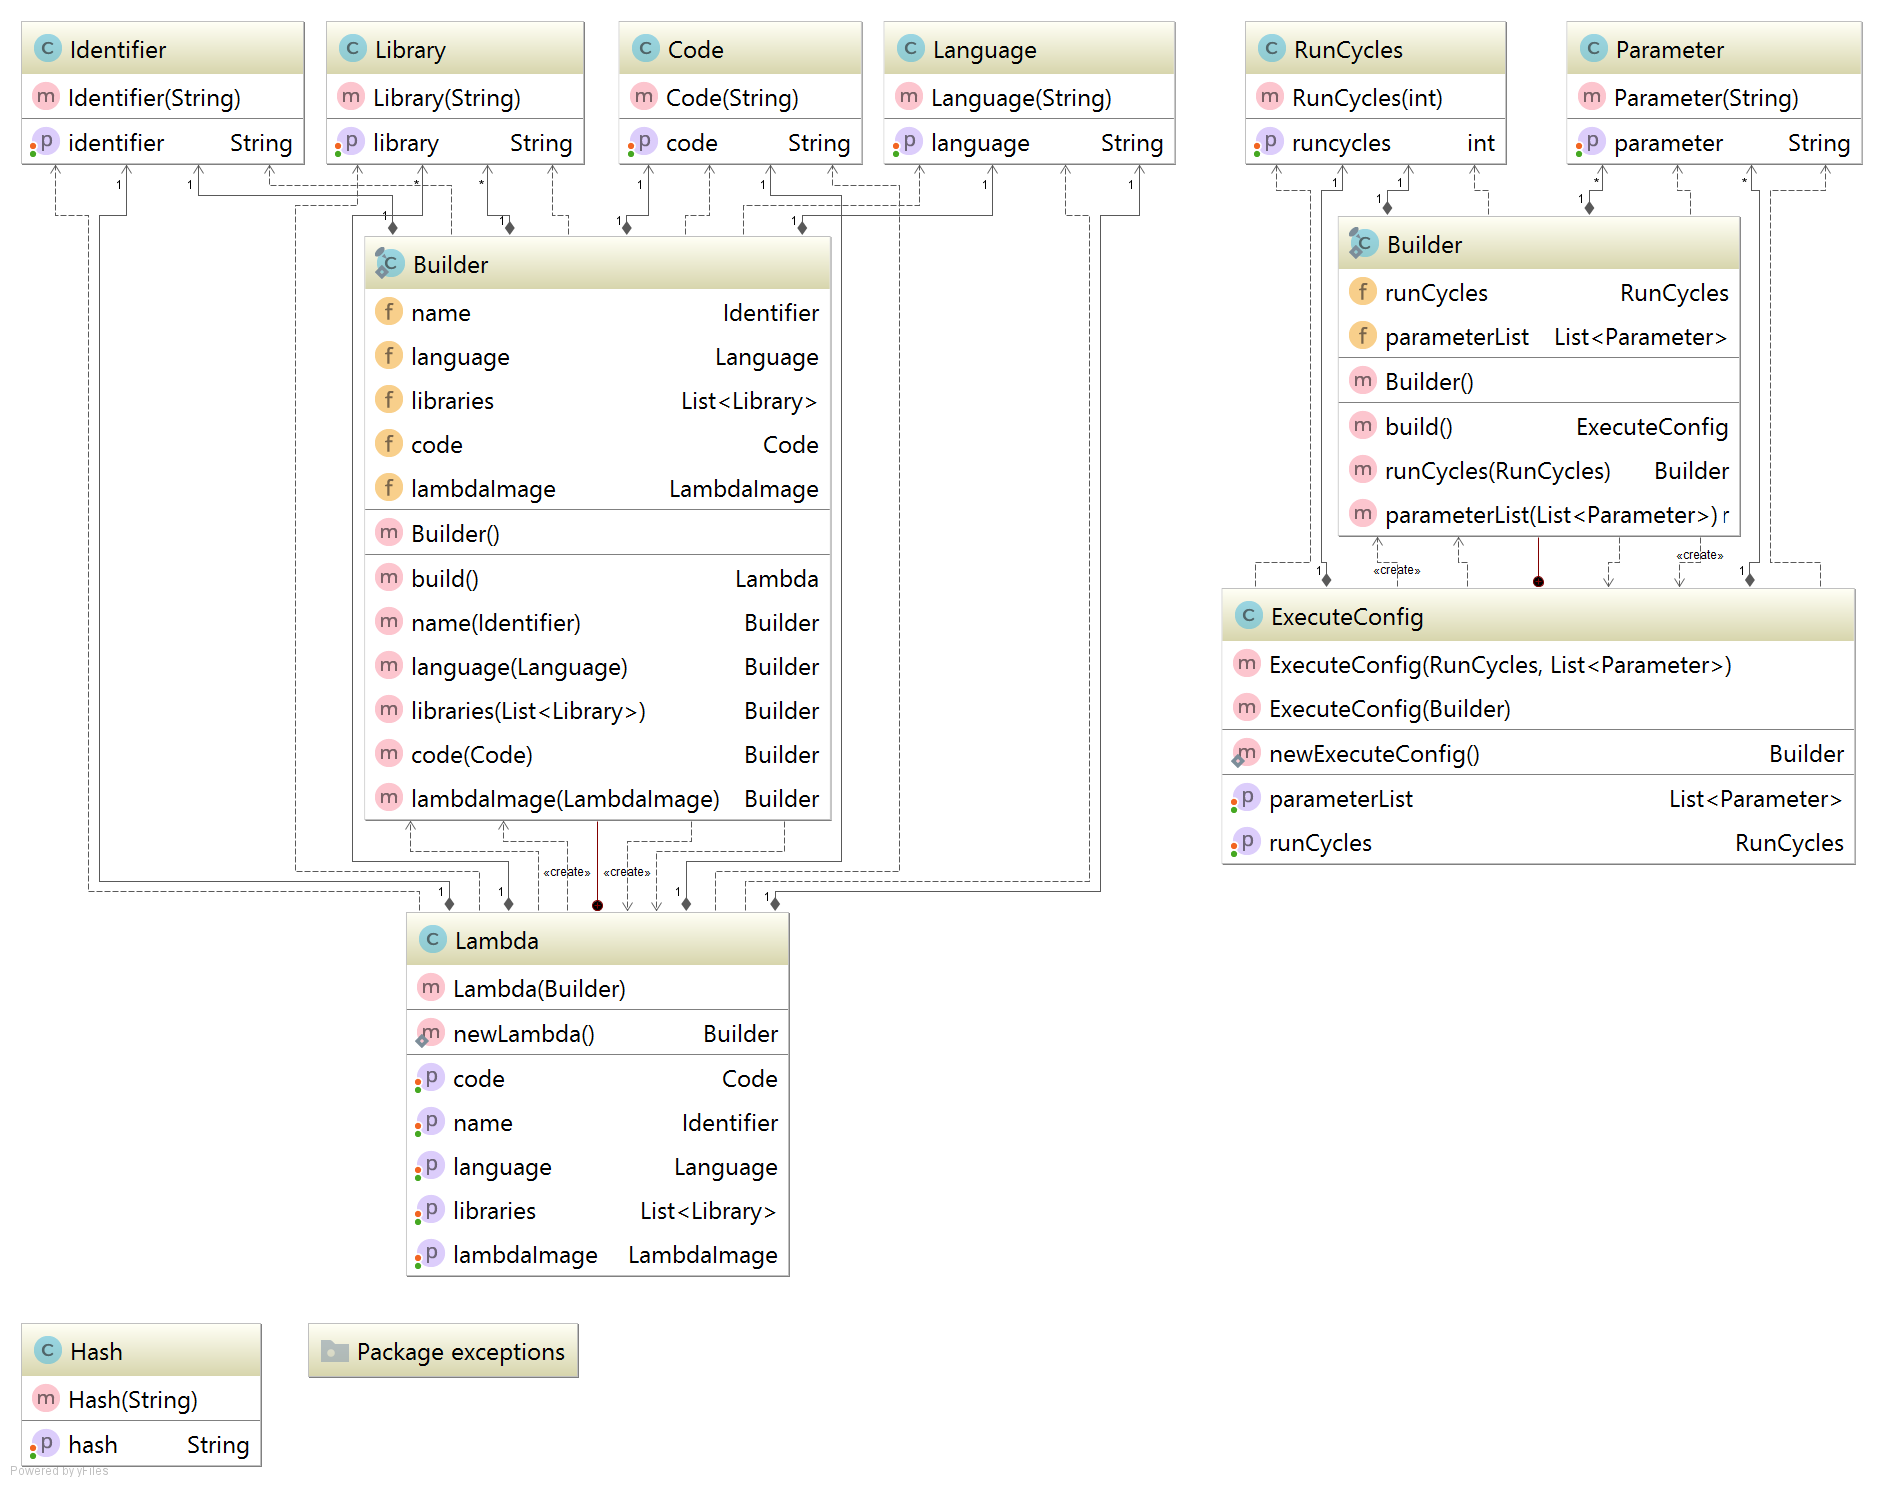
\includegraphics[width=18cm,height=20cm]{lambdadiagram}
	    \end{figure}
    \subsection{Messages}
	    \begin{figure}[!hb]
	    	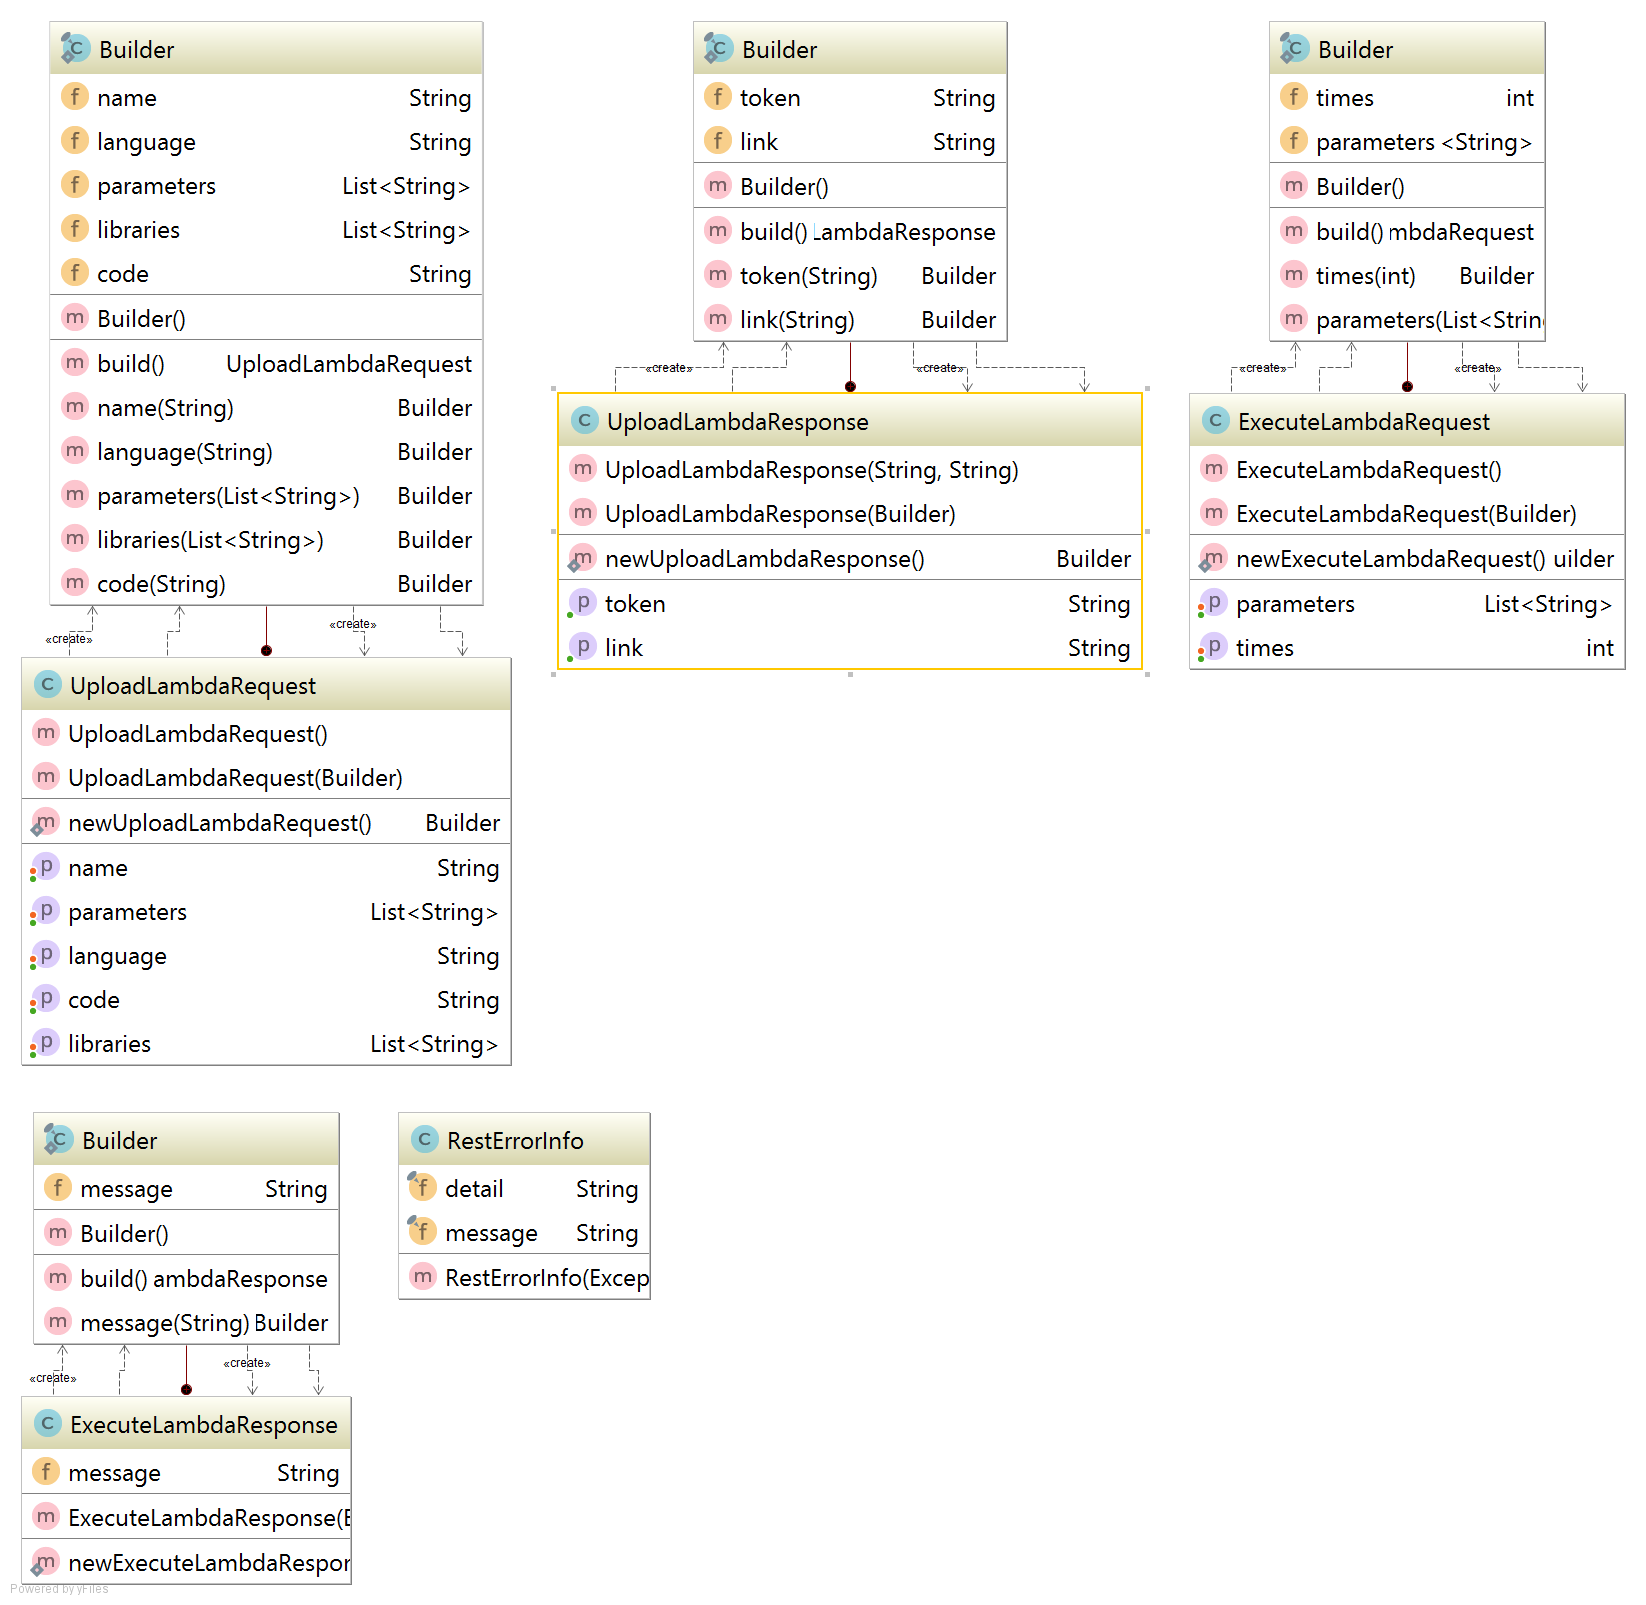
\includegraphics[width=18cm,height=20cm]{messagesdiagram}
	    \end{figure}
    \subsection{Auth}
	    \begin{figure}[!hb]
	    	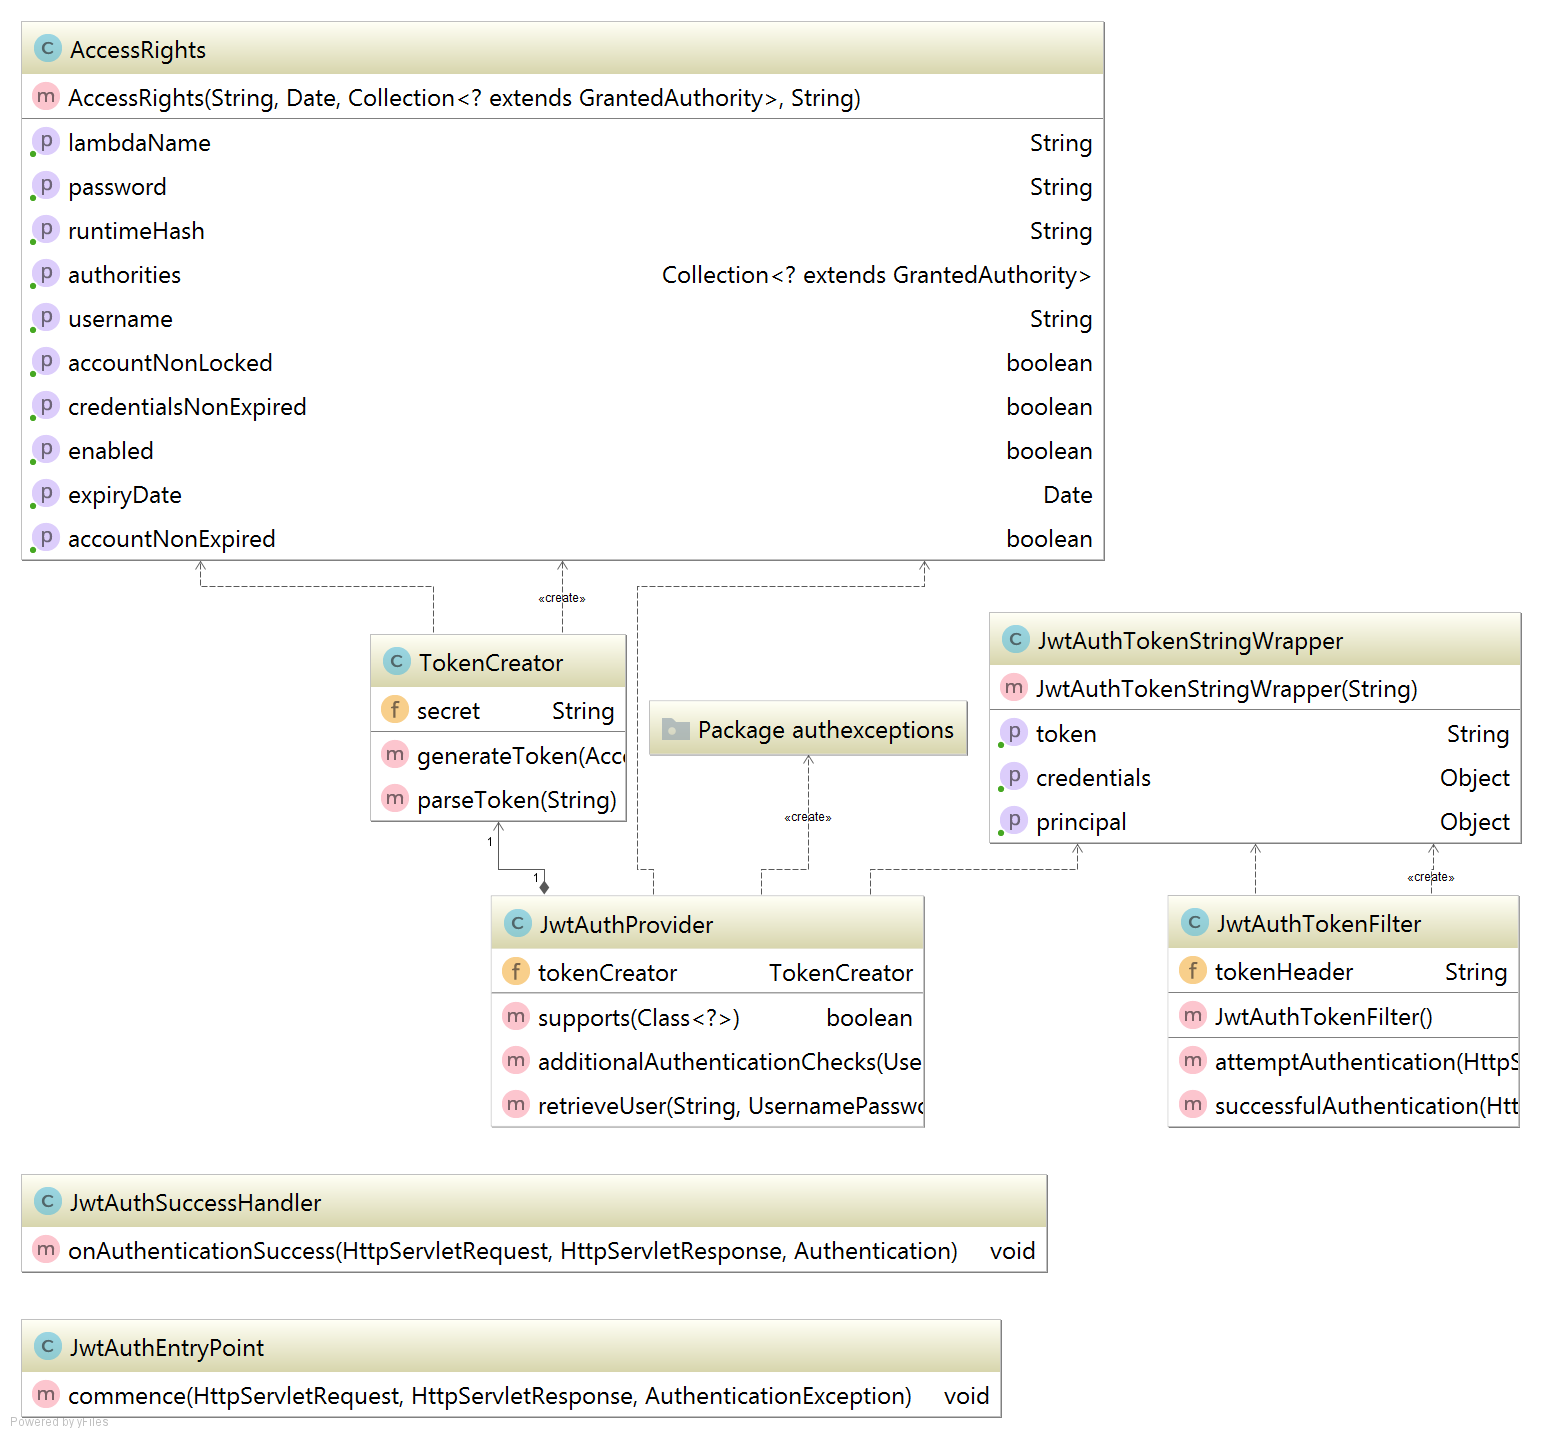
\includegraphics[width=18cm,height=20cm]{authdiagram}
	    \end{figure}
    \subsection{Runtime}
	    \begin{figure}[!hb]
	    	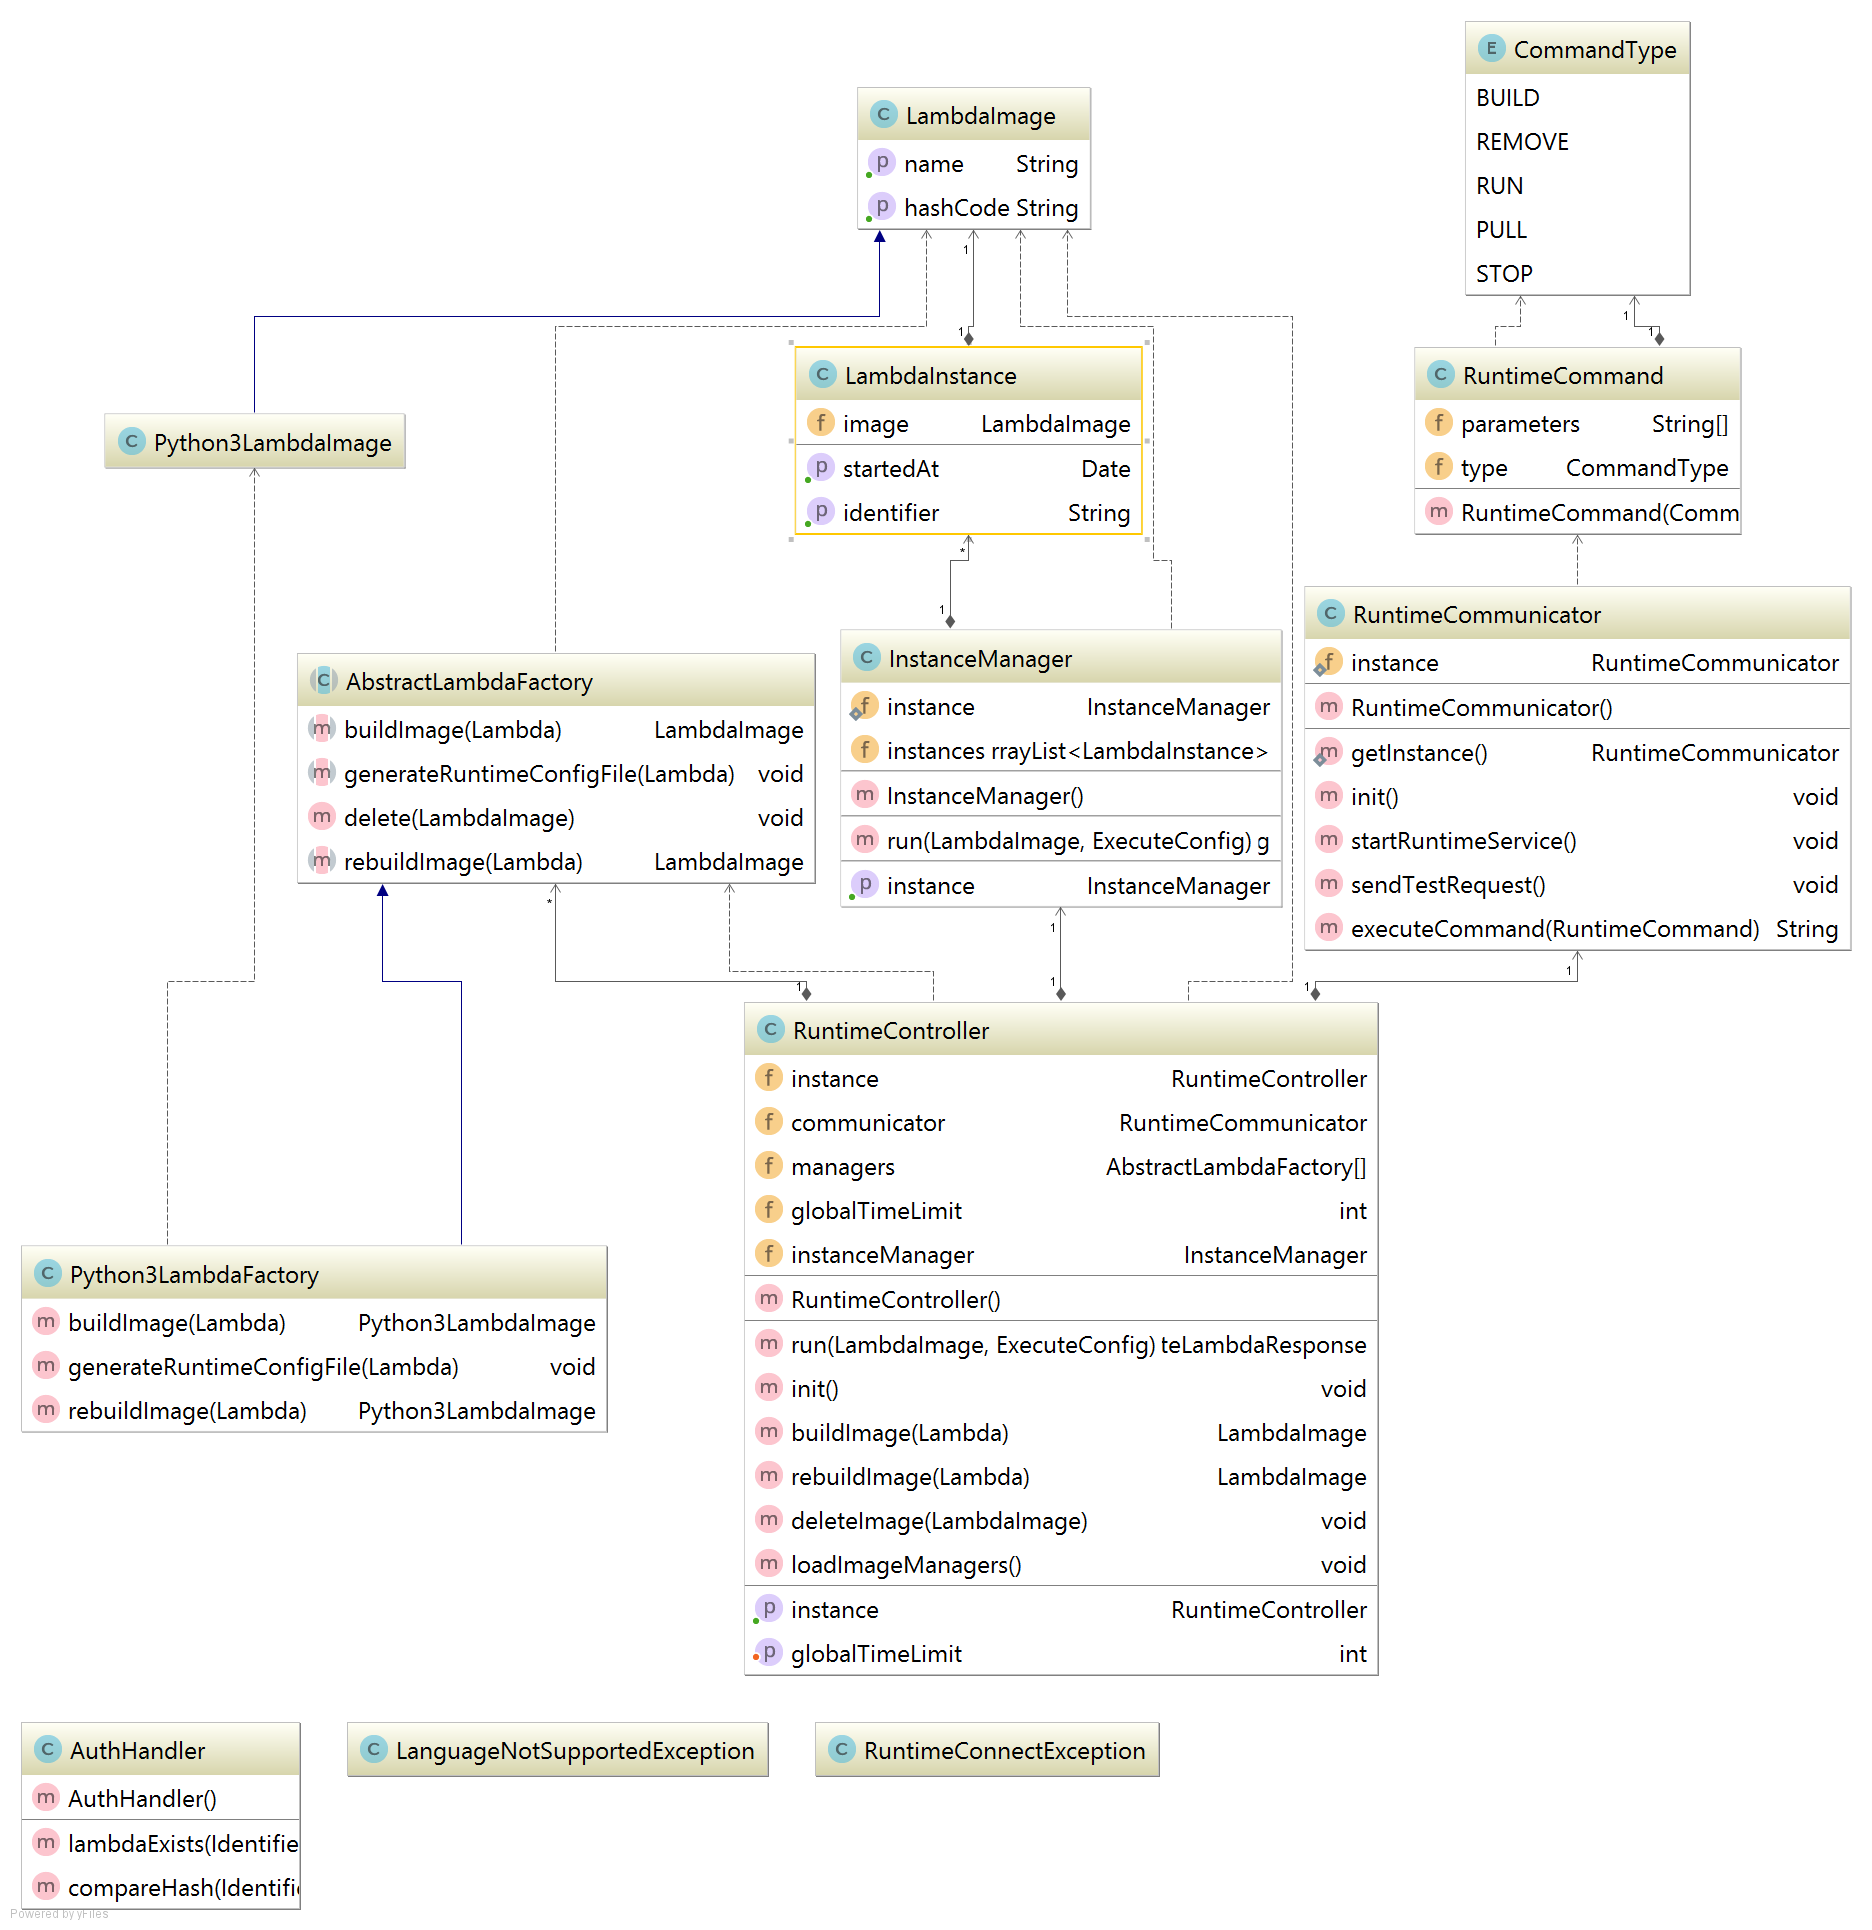
\includegraphics[width=18cm,height=20cm]{runtimediagram}
	    \end{figure}
    
    
		

	\section{Detaillierte Klassenbeschreibung: Start-und Konfigurationsklassen}
	\subsubsection{Application}
	\centering
	\begin{tabular}{|l|}
	\hline \\
	Application\\
	\hline 
	\\ 
	\hline \\
	+ main():void\\
	\hline 
	\end{tabular}
	
	\vspace{0.5cm}
	\raggedright
	Beschreibung:
	
	Main-Klasse zum Starten des Programms.
	
	\vspace{0.5cm}
	Attribute:
	\begin{itemize}
	\item keine
	\end{itemize}
	
	Methoden:
	\begin{itemize}
	\item main():void\linebreak
	Startet Spring und die SpringApplication.
	\end{itemize}
	
	\subsubsection{AuthenticationConfig}
	\centering
	\begin{tabular}{|l|}
	\hline \\
	AuthenticationConfig\\
	\hline \\
	- unauthorizedHandler:JwtAuthEntryPoint \\
	- authenticationProvider:JwtAuthProvider \\
	\hline \\
	+ authenticationManager():AuthenticationManager \\
	+ authenticationTokenFilterBean():JwtAuthTokenFilter\\
	+ configure(HttpSecurity httpSecurity):void \\
	\hline 
	\end{tabular}
		
	\vspace{0.5cm}
	\raggedright
	Beschreibung:
	
	Konfigurationsklasse für die Authentifizierung. Hier wird festgelegt, welche Pfade auf eine Authentifizierung gemappt werden und welche Rollen die Authentifizierungsmerkmale besitzen müssen, um eine Anfrage bearbeiten zu lassen.
	
	\vspace{0.5cm}
	Attribute:
	\begin{itemize}
	\item unauthorizedHandler:JwtAuthEntryPoint\linebreak
	JwtAuthEntryPoint Objekt zur Behandlung von nicht-authorisierten Anfragen
	\item authenticationProvider:JwtAuthProvider \linebreak
	JwtAuthProvider Objekt zur Prüfung der Authentifizierungsmerkmale
	\end{itemize}
	
	Methoden:
	\begin{itemize}
	\item  authenticationManager():AuthenticationManager \linebreak
	Gibt einen spezifizierten AuthenticationManager von Spring Security zurück. 
	\item authenticationTokenFilterBean():JwtAuthTokenFilter\linebreak
	Setzt die Klassen, mit denen Spring Security arbeiten soll.
	\item configure(HttpSecurity httpSecurity):void\linebreak
	Konfiguiert die Pfade für die Authentifizierung und die Rollen der Authentifizierungsmerkmale für die Pfade.
	\end{itemize}
	
	\section{Detaillierte Klassenbeschreibung: Model}
	\subsection{ServiceLayer: Service}
	\raggedright
	Für Service wird die Fassade als Entwurfsmuster 			benutzt. Die Fassade ist dafür gemacht, um die 					Funktionalität an andere Klassen des Subsystems zu 				delegieren und  dadurch den Umgang mit dem Subsystem zu 		vereinfachen. In unserem Fall wird die Fassade mit solchen 		Pakete wie lambda, messages, lambdaruntime, auth, 				converter und apicontroller arbeiten. 
	
	\subsubsection{LambdaFacade}
	
	\centering
	\begin{tabular}{|l|}
	\hline \\
	<<interface>> LambdaFacade \\
	\hline \\
	
	\hline \\

	+ upload(config: UploadLambdaRequest ): String\\
    + update(name: String, config: UploadLambdaRequest): String \\
    + getLambda(name: String): Lambda  \\
    + execute(name: String, config: ExecuteLambdaRequest): String \\
    +  deleteLambda(name: String ): String\\
    + authenticate(principal:Object):boolean\\
	\hline 
	
	\end{tabular}
	
	\vspace{0.5cm}
	\raggedright
	
	Beschreibung:
	
	Es ist eine Fassadeschnittstelle. Sie wird als Schnittstelle implementiert, um die Fassade flexibeler zu machen.
	
	\vspace{0.5cm}
	Attribute:
	\begin{itemize}
	\item keine
	
	\end{itemize}
	
	Methoden:
	\begin{itemize}
	\item  upload(config: UploadLambdaRequest ): String\linebreak
	Die Schnittstelle für das Hochladen von Lambdas. Muss 					implementiert werden, damit der Nutzer das Lambda an 			Serverless übergeben könnte.	
	
	\item update(name: String, config: UploadLambdaRequest): String \linebreak
	Die Schnittstelle für die Lambda Aktualisierung. Muss 			implementiert werden, damit der Nutzer das Lambda 				korrigieren oder ändern kann.
	
	\item getLambda(name: String): Lambda\linebreak
	Die Schnittstelle, damit der Nutzer die Lambda-Konfigurationen anschauen kann.
	
	\item execute(name: String, config: ExecuteLambdaRequest  ): String\linebreak
	Die Schnittstelle für die Lambda Ausführung. Muss 			implementiert werden, damit der Nutzer mit eingegebenen Parameter und Anzahl der Ausführungen das Lambda in Serverless ausführen kann. 
	\item deleteLambda(name: String ): String\linebreak
	Die Schnittstelle für die Entfernung von Lambdas. Muss 			implementiert werden, damit der Nutzer oder Serverless selbst nach einer definierten Zeit das Lambda löschen kann. 
	\item authenticate(principal:Object):boolean\linebreak
	Interface für die Authentifizierung. Muss implementiert werden, um den Hash aus dem Authentifizierungsmerkmal mit dem realen Image Hash zu checken. Garantiert das Vorhandensein eines zugehörigen Images. 	
	
	\end{itemize}
	\subsubsection{LambdaFacadeImpl}
	\centering
	\begin{tabular}{|l|}
	\hline \\
	LambdaFacadeImpl \\
	\hline \\
	- path: String \\	
	- maxTimes: int \\	
	- timeout: long\\
	- authHandler: AuthHandler \\
	- runTime: RuntimeController \\	
	\hline \\
	+ upload(config: UploadLambdaRequest): String\\
    + update(name: String, config: UploadLambdaRequest): String \\
    + getLambda(name: String): Lambda  \\
    + execute(name: String, config: ExecuteLambdaRequest): String \\
    +  deleteLambda(name: String ): String\\
    + authenticate(principal:Object):boolean\\
	\hline 
	\end{tabular}
	\vspace{0.5cm}
	
	
	\raggedright
	
	Beschreibung:
	
	Es ist eine Fassadeklasse. Sie bekommt die Aufgaben vom ApiController und verbindet sich mit den anderen Klassen, die in Fassade sind. 
	
	\vspace{0.5cm}
	Attribute:
	\begin{itemize}
	\item path: String\linebreak
	Die Directory, wo die LambdaImages gespeichert werden.
	\item maxTimes: int \linebreak
	\item timeout: long\linebreak
	\item authHandler: AuthHandler\linebreak
	\item runTime: RuntimeController\linebreak
	
	
	\end{itemize}
	
	Methoden:
	\begin{itemize}
	\item  upload(config: UploadLambdaRequest): String\linebreak
	Bekommt ein UploadLambdaRequest Objekt. Mit Hilfe der RequestServerConverter Methode wird ein Lambda Objekt aus einem UploadLambdaRequest Objekt erzeugt. Dann wird das Lambda Objekt an RuntimeController übergeben, um ein LambdaImage zu bauen.
	
	\item update(name: String, config: UploadLambdaRequest): String \linebreak
	Bekommt den Name eines Lambda, das aktualisiert werden soll, und ein UploadLambdaRequest Objekt. Mit Hilfe von RequestServerConverter Methode wird ein Lambda Objekt von ein UploadLambdaRequest Objekt erzeugt. Danach wird nach dem Lambda mit dem übergebenen Namen gesucht. Falls gefunden, wird das  Lambda gelöscht und das neue erzeugte Lambda an RuntimeController übergegeben.
	
	\item getLambda(name: String): Lambda\linebreak
	Es wird nach dem Lambda mit dem übergebenen Namen gesucht. Falls    gefunden, wird die getLambda Methode das gefundene Lambda zurückgeben.
	\item execute(name: String, config: ExecuteLambdaRequest): String\linebreak
	Bekommt den Namen eines Lambda, das ausgeführt sein soll, und ein ExecuteLambdaRequest Objekt. Mit Hilfe der RequestServerConverter Methode wird ein ExecuteConfig Objekt aus einem ExecuteLambdaRequest Objekt erzeugt. Danach wird nach dem Lambda mit dem übergebenen Namen gesucht. Falls gefunden, wird das Lambda  mit ExecuteConfig ausgeführt.
	\item deleteLambda(name: String ): String\linebreak
	Bekommt den Namen eines Lambda, das gelöscht werden soll. Es wird  nach dem Lambda mit dem übergebenen Namen gesucht. Falls gefunden, wird es gelöscht.
	
	\item authenticate(principal:Object):boolean\linebreak
	Parst ein AccessRights Objekt, ruft in der Runtime den AuthHandler auf, um den Hashcode und Identifier zu bekommen und prüft die Werte mit dem übergebenen Objekt.
	\end{itemize}

	
	
	
\subsection{ServiceLayer: LambdaRuntime}
	\subsubsection{AbstractLambdaFactory}
	\centering
	\begin{tabular}{|l|}
	\hline \\
	<<abstract>> AbstractLambdaFactory \\
	\hline \\
	
	\hline \\
	+ buildImage(lambda: Lambda): LambdaImage \\
	+ rebuildImage(lambda: Lambda): LambdaImage \\
	+ delete(image: LambdaImage): void \\
	\# <<abstract>> generateRuntimeConfigFile(lambda: Lambda) : void \\
	\hline 
	\end{tabular}
	
	\raggedright
	\vspace{0.5cm}
	
	Beschreibung: Die AbstrakteFabrik Klasse eines Abstrakte-Fabrik-Entwurfsmusters zur Erzeugung von LambdaImages.
	\vspace{0.5cm}	
	
	Attribute:
	\begin{itemize}
	\item keine
	\end{itemize}
	
	Methoden:
	\begin{itemize}
	\item buildImage(lambda: Lambda): LambdaImage
	\linebreak Gibt ein Befehl an RuntimeCommunikator um ein Image zu erzeugen.
	\item rebuildImage(lambda: Lambda): LambdaImage
	\linebreak Gibt ein Befehl an RuntimeCommunikator um alte Image zu löschen und ein neues zu bauen.
	\item delete(image: LambdaImage): void
	\linebreak Gibt ein Befehl an RuntimeCommunikator um ein Image zu löschen.
	\item generateRuntimeConfigFile(lambda: Lambda): void
	\linebreak
	Erzeugt Configaration für ein neues Image.
	\end{itemize}
		
	\subsubsection{CommandType}
	\centering
	\begin{tabular}{|l|}
	\hline \\
	<<enum>> CommandType \\
	\hline \\
	BUILD\\
    REMOVE\\
    RUN\\
    PULL\\
    STOP \\
	\hline 
	\end{tabular}
	
	\raggedright
	\vspace{0.5cm}
	
	Beschreibung: Enumeration für die verschiedenen Befehlstypen, die innerhalb der Runtime-Umgebung benötigt werden.
	
	\vspace{0.5cm}
	Konstanten:
	\begin{itemize}
	\item BUILD
	\linebreak bauen eines Images
	\item REMOVE
	\linebreak löschen eines Images
	\item RUN
	\linebreak starten einer Instanz eines Images
	\item PULL
	\linebreak download der für ein Image benötigten Komponenten
	\item STOP
	\linebreak stoppen einer Instanz
	\end{itemize}

	
	\subsubsection{InstanceManager}
	\centering
	\begin{tabular}{|l|}
	\hline \\
	InstanceManager \\
	\hline \\
	- \uline{instance: InstanceManager} \\
	- containers: ArrayList<Instance> \\
	\hline \\
	+ \uline{getInstance(): InstanceManager} \\
	+ run(LambdaImage image, ExecuteConfig config): String\\
	\hline 
	\end{tabular}
	
	\raggedright
	\vspace{0.5cm}
	
	Beschreibung:
	\linebreak
	Klasse zur Steuerung von Instanzen (starten, stoppen, \dots). Die Klasse wird als Singleton implementiert.
	\vspace{0.5cm}	
	
	Attribute:
	\begin{itemize}
	\item instance: InstanceManager
	\linebreak Eine Referenz auf das einzige Objekt der Klasse.
	\item containers: ArrayList<Instance>
	\linebreak Liste aller laufenden Instanzen.
	\end{itemize}
	
	Methoden:
	\begin{itemize}
	\item getInstance(): InstanceManager
	\linebreak Gibt die Referenz auf das einzige Objekt von InstanceManager zurück.
	\item run(LambdaImage image, ExecuteConfig config): String
	\linebreak Erzeugt ein neues Objekt der Klasse Instanz, fügt es zu instances hinzu und führt die Instanz aus.
	\end{itemize}
	
	\subsubsection{RuntimeCommand}
	\centering
	\begin{tabular}{|l|}
	\hline \\
	RuntimeCommand \\
	\hline \\
	- parameters: String[] \\
	- type: CommandType \\
	\hline \\
	\hline 
	\end{tabular}	
	
	\raggedright
	\vspace{0.5cm}
	
	Beschreibung:
	\linebreak Kapselung der Daten, die benötigt werden, um ein Kommando an die Runtime-Umgebung zu senden.
	\vspace{0.5cm}	
	
	Attribute:
	\begin{itemize}
	\item type: CommandType
	\linebreak Art des Befehls
	\item parameters: String[]
	\linebreak Eine Liste von Parameter zum Befehl.
	\end{itemize}		
	
	\subsubsection{RuntimeCommunicator}
	\centering
	\begin{tabular}{|l|}
	\hline \\
	RuntimeCommunicator \\
	\hline \\
	- \uline{instance: RuntimeCommunicator} \\
	\hline \\
	+ \uline{getInstance(): RuntimeCommunicator} \\
	+ init(): void \\
	- startRuntimeService(): void \\
	- sendTestRequest() : void \\
	+ sendCommand(command: RuntimeCommand): \\
	\hline 
	\end{tabular}
	
	\raggedright
	\vspace{0.5cm}
	
	Beschreibung:
	\linebreak Die RuntimeCommunicator-Klasse übernimmt die Kommunikation mit der verwendeten Runtime-Umgebung. Die Klasse wird als Singleton implementiert.
	\vspace{0.5cm}	
	
	Attribute:
	\begin{itemize}
	\item instance: RuntimeCommunicator
	\linebreak Eine Referenz auf das einzige Objekt der Klasse.
	\end{itemize}
	
	Methoden:
	\begin{itemize}
	\item getInstance(): RuntimeCommunicator
	\linebreak Gibt die Referenz auf das einzige Objekt von RuntimeCommunicator zurück.
	\item init(): void
	\linebreak Initialisiert die Runtime-Umgebung mithilfe startRuntimeService() und sendTestRequest().
	\item startRuntimeService(): void
	\linebreak Startet die Runtime-Umgebung
	\item sendTestRequest(): void
	\linebreak Prüft, ob die Runtime-Umgebung korrekt funktioniert, indem testweise eine Verbindung hergestellt wird.  
	\item sendCommand(command: RuntimeCommand): String
	\linebreak Sendet einen Befehl an die Runtime-Umgebung.
	\end{itemize}			
	
	\subsubsection{RuntimeController}
	\centering
	\begin{tabular}{|l|}
	\hline \\
	RuntimeController \\
	\hline \\
	- instance: RuntimeController \\
	- communicator: RuntimeCommunicator \\
	- factories: AbstractLambdaFactory[] \\
	- globalTimeLimit: int \\
	- instanceManager: InstanceManager \\
	\hline \\
	+ getInstance(): RuntimeController \\
	+ init(): void \\
	+ buildImage(lambda: Lambda): LambdaImage \\
	+ rebuildImage(lambda: Lambda): LambdaImage \\
	+ deleteImage(image: LambdaImage): void \\
	+ setGlobalTimeLimit(limit: int): void \\
	+ run(image: LambdaImage, config: ExecuteConfig): ExecuteLambdaResponce \\
	+ getInstance(): RuntimeController \\
	- loadImageFactories(): void \\
	\hline
	\end{tabular}		
	
	\raggedright
	\vspace{0.5cm}	
	
	Beschreibung:
	\linebreak Die Klasse RuntimeController ist eine Fassade, die alle Details des Runtime-Systems versteckt. Alle Methoden rufen nur die Methoden in den jeweils zuständigen Klassen auf. Die Klasse wird als Singleton implementiert. 
	\vspace{0.5cm}	
	
	Attribute:
	\begin{itemize}
	\item instance: RuntimeController
	\linebreak Eine Referenz auf das einzige Objekt der Klasse.
	\item communicator: RuntimeCommunicator
	\linebreak Eine Referenz auf den RuntimeCommunicator.
	\item factories: AbstractLambdaFactory[]
	\linebreak Die Fabriken zur Erzeugung von Lambdas.
	\item globalTimeLimit: int
	\linebreak Die maximale Laufzeit einer LambdaFunktion.
	\item instanceManager: InstanceManager
	\linebreak Die Referenz auf den InstanceManager.
	\end{itemize}
	
	Methoden:
	\begin{itemize}
	\item getInstance(): RuntimeController
	\linebreak Gibt die Referenz auf das einzige Objekt von RuntimeController zurück.
	\item init(): void
	\linebreak Initialisiert das Runtime-System.
	\item buildImage(lambda: Lambda): LambdaImage
	\linebreak leitet den Aufruf weiter an die entsprechende ImageFactory.
	\item rebuildImage(lambda: Lambda): LambdaImage
	\linebreak leitet den Aufruf weiter an die entsprechende ImageFactory.
	\item deleteImage(image: LambdaImage): void
	\linebreak leitet den Aufruf weiter an die entsprechende ImageFactory.
	\item setGlobalTimeLimit(limit: int)
	\linebreak setzt eine maximal Ausführungszeit für ein Lambda.
	\item run(image: LambdaImage, config: ExecuteConfig): ExcuteLambdaResponse
	\linebreak leitet den Aufruf weiter an den InstanceManager.
	\item loadImageFactories(): void
	\linebreak lädt und initialisiert die ImageFactory für jede unterstützte Sprache.
	\end{itemize}			
	
	\subsubsection{LambdaImage}
	\centering
	\begin{tabular}{|l|}
	\hline \\
	<<abstract>> LambdaImage \\
	\hline \\
	- name: String \\
	- hashCode: long \\
	\hline \\
	\hline 
	\end{tabular}
	
	\raggedright
	\vspace{0.5cm}	
	
	Beschreibung: 
	\linebreak Abstrakte Klasse für die Speicherung von Informationen über die angelegten Lambdas. Enthält die Informationen, die zum Starten einer Instanz notwendig sind.
	\vspace{0.5cm}
	
	Attribute:
	\begin{itemize}
	\item identifier: String
	\linebreak Der Identifikator für ein Image innerhalb der Runtime-Umgebung.
	\item hashCode: long
	\linebreak Der HashCode, der dem Image innerhalb der Runtime-Umgebung zugeordnet wurde.
	\end{itemize}
	
	Methoden:
	\begin{itemize}
	\item keine
	\end{itemize}	
		
	\subsubsection{LambdaInstance}
	\centering
	\begin{tabular}{|l|}
	\hline \\
	LambdaInstance \\
	\hline \\
	- image: LambdaImage \\
	- identifier: String \\
	- startedAt: Date \\
	\hline \\
	\hline 
	\end{tabular}
	
	\raggedright
	\vspace{0.5cm}	
	
	Beschreibung: Eine laufende Instanz einer Lambda-Funktion.
	\vspace{0.5cm}
	
	Attribute:
	\begin{itemize}
	\item image: LambdaImage
	\linebreak Eine Referenz auf das zugehörige Image der laufenden Instanz
	\item identifier: String
	\linebreak Der Identifikator für eine laufende Instanz innerhalb der Runtime-Umgebung.
	\item startetAt: Date
	\linebreak Der Zeitpunkt, an dem die Instanz gestartet wurde. Wird benötigt, um die Instanz bei Überschreiten des Zeitlimits abbrechen zu können.
	\end{itemize}
	
	Methoden:
	\begin{itemize}
	\item keine
	\end{itemize}
		
		
	\subsubsection{Python3LambdaImage und Python3LambdaFactory}
	Beschreibung: 
	\linebreak Diese beiden Klassen sind Teil des AbstrakteFabrik-Entwurfsmusters zur Produktion von LambdaImages. Python3LambdaImage und Python3LambdaFactory sind die nicht-abstrakte Fabrik und das nicht-abstrakte LambdaImage für Lambdas in der Programmiersprache Python (Version 3).
	\linebreak
	Die Verwendung von Python3 wird unterstützt. Die Software kann um weitere Sprachen erweitert werden. Dafür müssen für jede Sprache eine Unterklasse von AbstractLambdaFactory und von LambdaImage implementiert werden (z. B. JavaScriptLambdaFactory und JavaScriptLambdaImage).
	
	\subsubsection{AuthHandler}
	\centering
	\begin{tabular}{|l|}
	\hline \\
	AuthHandler \\
	\hline \\

	\hline \\
	+ lambdaExists(name:Identifier):boolean \\
	+ compareHash(name:Identifier, hash:Hash):boolean\\
	\\ \hline
	\end{tabular}
	
	\raggedright
	\vspace{0.5cm}
	Beschreibung:
	
	Klasse zur Bereitstellung von Information über die Runtime für die finale Authentifizierung.
	
	\vspace{0.5cm}
	Attribute:
	\begin{itemize}
	\item keine
	\end{itemize}
	
	Methoden:
	\begin{itemize}
	\item compareHash(name:Identifier, hash:Hash):boolean\linebreak
	Vergleicht bekommenen Hash mit dem des RuntimeImages unter bestimmten Namen.
	\item lambdaExists(name:Identifier):boolean \linebreak
	Prüft, ob ein Lambda mit dem Namen vorhanden ist.
	\end{itemize}
	
	
	\subsubsection{Exceptions}
	\centering
	\begin{tabular}{|l|}
	\hline \\
	LanguageNotSupportedException \\ \hline
	\\ \hline
	\end{tabular}
	
	\raggedright
	\vspace{0.5cm}
	Beschreibung:
	\linebreak Exception-Klasse für die Angabe ungültiger Parameter für die Sprache eines Lambdas.
	
	\vspace{0.5cm}
	
	\centering
	\begin{tabular}{|l|}
	\hline \\
	RuntimeConnectException\\ \hline
	\\ \hline
	\end{tabular}	
	
	\raggedright
	\vspace{0.5cm}
	Beschreibung:
	\linebreak Exception-Klasse für Fehler, die mit der Runtime-Umgebung zusammenhängen (v.a. Verbindungsfehler)
	
	\vspace{0.5cm}	
	
	
	\subsection{Exception}
	\subsubsection{LambdaExceptions}
	\centering
	\begin{tabular}{|l|}
	\hline \\
	LambdaNotFoundException\\ \hline
	\\ \hline
	\end{tabular}
	
	\raggedright
	\vspace{0.5cm}	
	
	Beschreibung:
	
	Exception, falls das Lambda nicht gefunden wird.
	
	
	\centering
	\begin{tabular}{|l|}
	\hline \\
	LambdaDuplicatedNameException\\ \hline
	\\ \hline
	\end{tabular}
	
	\raggedright
	\vspace{0.5cm}	
	
	Beschreibung:
	
	Exception, falls ein Lambda mit gleichem Namen schon existiert.
	
	\subsection{Converter}
	\subsubsection{RequestServerConverter}
	\centering
	\begin{tabular}{|l|}
	\hline \\
	RequestServerConverter\\
	\hline \\
    \hline \\
    + uploadToLambda(uploadRequest: UploadLambdaRequest ):Lambda \\
	+ executeToConfig(executeRequest: ExecuteLambdaRequest ):ExecuteConfig\\
	+ lambdaToUpload(lambda: Lambda):UploadLambdaRequest\\	
	\hline 
	\end{tabular}
	
	\raggedright
	\vspace{0.5cm}
	Beschreibung:
	
	Die Klasse macht die Syntax Überprüfung. Sie verbindet die lambda Pakete und die messages Pakete.
	
	\vspace{0.5cm}
	Attribute:
	\begin{itemize}
	\item keine \linebreak
    
	\end{itemize}
	
	Methoden:
	\begin{itemize}
	\item uploadToLambda(uploadRequest: UploadLambdaRequest ):Lambda\linebreak
	Erzeugt ein Lambda Objekt aus einem UploadLambdaRequest Objekt.
	\item executeToConfig(executeRequest: ExecuteLambdaRequest ):ExecuteConfig \linebreak
	Erzeugt ein ExecuteConfig Objekt aus einem ExecuteLambdaRequest Objekt.
	\item lambdaToUpload(lambda: Lambda):UploadLambdaRequest \linebreak
	Erzeugt ein UploadLambdaRequest Objekt aus einem Lambda Objekt.
	\end{itemize}
	
	
	\subsection{Lambda}
		\subsubsection{Lambda}
		\centering
	\begin{tabular}{|l|}
	\hline \\
	Lambda\\
	\hline \\
	- name: Identifier\\
    - language: Language\\
    - libraries: List<Library>\\
    - code: Code\\
    - lambdaImage: LambdaImage\\
    \hline \\
	\hline 
	\end{tabular}
	
	\raggedright
	\vspace{0.5cm}
	Beschreibung:
	
	Klasse zur objektorientierten Modellierung der Lambda-Funktion.
	
	\vspace{0.5cm}
	Attribute:
	\begin{itemize}
	\item name: Identifier \linebreak
	Name der Funktion.
    \item language: Language \linebreak
    Sprache der Funktion.
    \item libraries: List<Library> \linebreak
    Libraries, die die Funktion zur Ausführung benötigt.
    \item code: Code \linebreak
    Die Funktion selbst.
    \item lambdaImage: LambdaImage\linebreak
    Eine Referenz auf das zugehörige Image der Lambda.
    
	\end{itemize}
	
	Methoden:
	\begin{itemize}
	\item keine
	\end{itemize}
	
	\subsubsection{Code}
		\centering
	\begin{tabular}{|l|}
	\hline \\
	Code\\
	\hline \\
    - code: String\\
    \hline \\
	\hline 
	\end{tabular}
	
	\raggedright
	\vspace{0.5cm}
	Beschreibung:
	
	Klasse zur Verpackung der Code von der Lambda-Funktion.
	
	\vspace{0.5cm}
	Attribute:
	\begin{itemize}
    \item code: String \linebreak
    Der Code der Funktion als String.
	\end{itemize}
	
	Methoden:
	\begin{itemize}
	\item keine
	\end{itemize}
	
	\subsubsection{ExecuteConfig}
		\centering
	\begin{tabular}{|l|}
	\hline \\
	ExecuteConfig\\
	\hline \\
	- runCycles: RunCycles\\
    - parameterList: List<Parameter>\\
   
    \hline \\
	\hline 
	\end{tabular}
	
	\raggedright
	\vspace{0.5cm}
	Beschreibung:
	
	Klasse zur Verpackung der Ausführungskonfigurationen.
	
	\vspace{0.5cm}
	Attribute:
	\begin{itemize}
	\item runCycles: RunCycles \linebreak
	Wie oft die Funktion ausgeführt werden muss.
    \item parameterList: List<Parameter> \linebreak
    Parameter, die die Funktion zur Ausführung benötigt.
	\end{itemize}
	
	Methoden:
	\begin{itemize}
	\item keine
	\end{itemize}
	
	\subsubsection{Identifier}
		\centering
	\begin{tabular}{|l|}
	\hline \\
	Identifier\\
	\hline \\
	- identifier: String\\
    \hline \\
	\hline 
	\end{tabular}
	
	\raggedright
	\vspace{0.5cm}
	Beschreibung:
	
	Klasse zur Verpackung des Funktionsnamens.
	
	\vspace{0.5cm}
	Attribute:
	\begin{itemize}
	\item identifier: String \linebreak
	Name der Funktion.
    
	\end{itemize}
	
	Methoden:
	\begin{itemize}
	\item keine
	\end{itemize}
	
	\subsubsection{Language}
		\centering
	\begin{tabular}{|l|}
	\hline \\
	Language\\
	\hline \\
    - language: String\\
    \hline \\
	\hline 
	\end{tabular}
	
	\raggedright
	\vspace{0.5cm}
	Beschreibung:
	
	Klasse zur Verpackung einer Programmiersprache.
	
	\vspace{0.5cm}
	Attribute:
	\begin{itemize}
    \item language: String \linebreak
    Sprache der Funktion.
	\end{itemize}
	
	Methoden:
	\begin{itemize}
	\item keine
	\end{itemize}
	
	\subsubsection{Library}
		\centering
	\begin{tabular}{|l|}
	\hline \\
	Library\\
	\hline \\
	- library: String\\
   
    \hline \\
	\hline 
	\end{tabular}
	
	\raggedright
	\vspace{0.5cm}
	Beschreibung:
	
	Klasse zur Verpackung einer Bibliothek.
	
	\vspace{0.5cm}
	Attribute:
	\begin{itemize}
    \item library: String \linebreak
    Name der Bibliothek als String.
	\end{itemize}
	
	Methoden:
	\begin{itemize}
	\item keine
	\end{itemize}
	
	\subsubsection{Parameter}
		\centering
	\begin{tabular}{|l|}
	\hline \\
	Parameter\\
	\hline \\
	- parameter: String\\
   
    \hline \\
	\hline 
	\end{tabular}
	
	\raggedright
	\vspace{0.5cm}
	Beschreibung:
	
	Klasse zur Verpackung eines Parameters der Lambda-Funktion.
	
	\vspace{0.5cm}
	Attribute:
	\begin{itemize}
	\item parameter: String \linebreak
	Ein Parameter als String.
	\end{itemize}
	
	Methoden:
	\begin{itemize}
	\item keine
	\end{itemize}
	
	\subsubsection{RunCycles}
		\centering
	\begin{tabular}{|l|}
	\hline \\
	RunCycles\\
	\hline \\
	- runcycles: int\\
   
    \hline \\
	\hline 
	\end{tabular}
	
	\raggedright
	\vspace{0.5cm}
	Beschreibung:
	
	Klasse zur Verpackung der Anzahl der Ausführungszyklen
	
	\vspace{0.5cm}
	Attribute:
	\begin{itemize}
	\item runCycles: int \linebreak
	Wie oft die Funktion ausgeführt wird.
	\end{itemize}
	
	Methoden:
	\begin{itemize}
	\item keine
	\end{itemize}
	
	\subsection{Messages}
	\subsubsection{ExecuteLambdaRequest}
		\centering
	\begin{tabular}{|l|}
	\hline \\
	ExecuteLambdaRequest\\
	\hline \\
	- times: int\\
    - parameters: List<String>\\
   
    \hline \\
	\hline 
	\end{tabular}
	
	
	\vspace{0.5cm}
	\raggedright
	
	Beschreibung:	
	
	Enthält die in Java Attribute geparste JSON Datei, die die Anfrage zum Ausführen enthält.
	\vspace{0.5cm}
	
	Attribute:
	\begin{itemize}
	\item time: int\linebreak
	Die Anzahl von Ausführungen.
	\item parameters: List<String> \linebreak	
	Die Liste von Typen, welche die Parameter bei der Ausführung haben.  
	\end{itemize}
	
	Methoden:
	\begin{itemize}
	\item keine
	\end{itemize}
	\subsubsection{ExecuteLambdaResponse}
		\centering
	\begin{tabular}{|l|}
	\hline \\
	ExecuteLambdaResponse\\
	\hline \\
	- message: String\\
    \hline \\
	\hline 
	\end{tabular}
	
	
	\vspace{0.5cm}
	\raggedright
	
	Beschreibung:
		
	Enthält die in Java Attribute geparste JSON Datei, die die Antwort nach dem Ausführen enthält.
	\vspace{0.5cm}
	
	Attribute:
	\begin{itemize}
	\item message: String\linebreak
	Die Antwort, die der Nutzer nach der Ausführung bekommt.
		
	\end{itemize}
	
	Methoden:
	\begin{itemize}
	\item keine
	\end{itemize}
	\subsubsection{UploadLambdaRequest}
		\centering
	\begin{tabular}{|l|}
	\hline \\
	UploadLambdaRequest\\
	\hline \\
	- name: String\\	
    - language: String\\    
    - libraries: List<String>\\    
    - code: String\\
    \hline \\
	\hline 
	\end{tabular}
	
	
	\vspace{0.5cm}
	\raggedright
	
	Beschreibung:	
	
	Enthält die in Java Attribute geparste JSON Datei, die die Anfrage zum Hochladen enthält.
	\vspace{0.5cm}
	
	Attribute:
	\begin{itemize}
	\item name: String\linebreak
	Der Name des Lambda.	
	\item language: String\linebreak
	Die Programmiersprache des Lambda.	
	\item libraries: List<String>\linebreak	
	Die Liste von Biblioteken.
	\item code: String\linebreak
	Der Code des Lambda als String.	
	\end{itemize}
	
	Methoden:
	\begin{itemize}
	\item keine
	\end{itemize}
	\subsubsection{UploadLambdaResponse}
		\centering
	\begin{tabular}{|l|}
	\hline \\
	UploadLambdaResponse\\
	\hline \\
	- token: String\\	
	- link: String\\
    \hline \\
	\hline 
	\end{tabular}
	
	\vspace{0.5cm}
	\raggedright
	
	Beschreibung:
		
	Enthält die in Java Attribute geparste JSON Datei, die die Antwort nach dem Hochladen enthält.
	\vspace{0.5cm}
	
	Attribute:
	\begin{itemize}
	\item token: String\linebreak
	Der Token, der für die weitere Authentifizierung benutzt wird.	
	\item link: String\linebreak
	Der Link, unter dem das Lambda gespeichert wird.	
	\end{itemize}
	
	Methoden:
	\begin{itemize}
	\item keine
	\end{itemize}
	
	
	
	\subsubsection{RestErrorInfo}
    \centering
	\begin{tabular}{|l|}
	\hline \\
	RestErrorInfo\\
	\hline \\
	- detail: String\\
	- message: String\\
    \hline \\
	\hline 
	\end{tabular}
	
	\vspace{0.5cm}
	\raggedright
	
	
	Beschreibung:
	
	Die Klasse verallgemeinert die Ausgabe von Exceptions.	
	
	\vspace{0.5cm}
	
	Attribute:
	\begin{itemize}
	\item detail: String\linebreak
	Die Nachricht von Exception.
	\item message: String\linebreak	
	Die Nachricht für Entwickler.
	\end{itemize}
	
	
	\subsubsection{Hash}
		\centering
	\begin{tabular}{|l|}
	\hline \\
	Hash\\
	\hline \\
	- hash: String\\
    \hline \\
	\hline 
	\end{tabular}
	
	
	\vspace{0.5cm}
	\raggedright
	
	Beschreibung:	
	
	Wrapperklasse für den Hashcode. Nur benötigt für Authentifizierung.
	
	\vspace{0.5cm}
	Attribute:
	\begin{itemize}
	\item hash: String\linebreak	
	Enthält den Hash
	\end{itemize}
	
	Methoden:
	\begin{itemize}
	\item Getter und Setter
	\end{itemize}
	
	
	\newpage
	\section{Detaillierte Klassenbeschreibung: Auth}
	\raggedright
		Die Authentifizierung besteht aus zwei Teilen. Dieser Auth Teil beschreibt das Zusammenspiel mit Spring Security, welches vor dem Eintritt in die Fassade passiert. Hier wird das übergebene JSON Webtoken auf Syntax und zeitliche Gültigkeit geprüft. 
		
		Die Konfiguration der REST Pfade, auf der die Authentifizierung gelten soll findet außerhalb des Pakets in AuthenticationConfig statt. 

		Der zweite Teil hinter der Fassade geschieht mit Zusammenspiel der Runtime und der Fassadenklasse. Diese prüfen die Werte aus dem Token (z.B. Hashcode) mit den zugehörigen Images und erlauben Zutritt bei korrekten Werten. Hier wird nur der erste Teil beschrieben.
		
	\begin{figure}[!hb]
    \includegraphics[width=17cm,height=12cm]{authpaket}
	\end{figure}

	\subsubsection{JwtAuthTokenFilter}
\centering
	\begin{tabular}{|l|}
	\hline \\
	JwtAuthTokenFilter\\ \hline \\
	- tokenHeader: String\\
	 \hline \\
	+ attemptAuthentification(request:HttpServletRequest, response:HttpServletResponse): Authentification\\
	\# successfulAuthentification(request:HttpServletRequest, response:HttpServletResponse,\\ chain:FilterChain, authResult:Authentication): void\\

	 \hline
	\end{tabular}
		 
	\vspace{0.7cm}
	\raggedright
	Beschreibung:

	Kümmert sich um den Beginn der Authentifizierung und um die Weiterleitung der Anfrage bei erfolgreicher Authentifizierung. Im Fall einer nicht erfolgreichen Authentifizierung werden in der Oberklasse AbstractAuthenticaionProcessingFilter von Spring Security behandelt. Für Näheres dazu siehe die Spring Security Dokumentation.
	
	\vspace{0.5cm}
	Attribute:
	\begin{itemize}
	\item tokenHeader: String \linebreak
	Der Wert unter dem Eintrag jwt.header aus der Datei application.yml im Ordner resources wird gelesen und mithilfe von Spring in das Attribut geschrieben. Es beschreibt die Header in der REST-Anfrage, die als Authorisierungsmerkmal akzeptiert werden. Empfohlen ist "\ Authorization"\ unter diesem Eintrag.
	\end{itemize}
	
	Methoden:
	\begin{itemize}
	\item attemptAuthentification(request:HttpServletRequest, response:HttpServletResponse): Authentification\linebreak
	Beginn des Authentifizierungsablaufs. Spring füttert die Methode mit den Parametern und ruft diese auf. Erstellt wird in der Methode ein Objekt JwtTokenStringWrapper, welches den übergebenen Token als Objekt darstellt, ruft mithilfe des AbstractAuthenticationProcessingFilters den AuthenticationManager von Spring auf und authentifiziert mithilfe dessen und dem JwtTokenStringWrapper Objekt die Anfrage. Als Rückgabe wird ein Authentification-Objekt übergeben, welches genauer spezifiziert ein Objekt der Klasse AccessRights ist. Da diese Methode eine Methode der Oberklasse überschreibt, kann dieses jedoch nicht so genau spezifiziert werden.
	\item successfulAuthentification(request:HttpServletRequest, response:HttpServletResponse, chain:FilterChain, authResult:Authentication): void\linebreak
	Falls die Authentifizierung erfolgreich war, wird diese Methode von Spring aufgerufen. Die Methode führt den Anfragenfluss fort, als wäre keine Authentifizierung da gewesen.
	\end{itemize}	
	
	\subsubsection{AccessRights}
\centering
	\begin{tabular}{|l|}
	\hline \\
	AccessRights \\ \hline \\
	- lambdaName:String\\
	- expiryDate:Date\\
	- authorities:Collection<? extends GrantedAuthority>\\
	- runtimeHash:String
	\\ 
	\hline \\
	+ AccessRights(lambdaName:String, expiryDate:Date, \\ authorities:Collection<? extends GrantedAuthority>, dockerHash:String) \\
	+ getUsername():String\\
	+ getPassword():String \\
	+ isAccountNonLocked():boolean\\
	+ isCredentialsNonExpired():boolean\\
	+ isEnabled():boolean\\ 
	+ isAccountNonExpired():boolean\\
 \\ \hline
	\end{tabular}
 
	\vspace{0.5cm}
	\raggedright
	Beschreibung:
	
	Implementierung des Spring Security Interfaces UnserDetails. Wird erstellt nach der Prüfung des Authentifizierungsmerkmals in TokenCreator, um ein Objekt zu haben, das den Status eines Merkmals angibt und mit dem in der Abfolge weitergearbeitet werden kann.
	
	\vspace{0.5cm}
	Attribute:
	\begin{itemize}
	\item lambdaName:String \linebreak
	Name der Lambdafunktion (Identifier).
	\item authorities:Collection<? extends GrantedAuthority> \linebreak
	Objekte der Klasse GrantedAuthority, die in dem Subtoken (SUB) oder Mastertoken (MASTER) aus den Werten des Authentifizierungsmerkmals generiert werden
	\item runtimeHash:String \linebreak
	Hash des Runtime Images, übergeben vom Authentifizierungsmerkmal. Wird später mit dem realen Hash des Images unter dem gegebenen Namen entgegengeprüft.
	\item expiryDate:Date \linebreak
	Datum, an dem das Authentifizierungsmerkmal ungültig wird.
	\end{itemize}
	
	Methoden:
	\begin{itemize}
	\item AccessRights(lambdaName:String, expiryDate:Date, authorities:Collection<? extends GrantedAuthority>, dockerHash:String) \linebreak
	Konstruktor
	\item getUsername():String\linebreak
	Stummelmethode. Gibt immer null zurück.
	\item getPassword():String \linebreak
	Stummelmethode. Gibt immer null zurück.
	\item isAccountNonLocked():boolean \linebreak
	Stummelmethode. Gibt immer true zurück.
	\item isCredentialsNonExpired():boolean\linebreak
	Prüft, ob der Wert von expiryDate vor dem aktuellem Datum liegt. Gibt true zurück, falls dies der Fall ist, sonst false.
	\item isEnabled():boolean\linebreak
	Stummelmethode. Gibt immer true zurück.
	\item isAccountNonExpired():boolean \linebreak
	Stummelmethode. Gibt immer true zurück.
	\item Getter und Setter
	\end{itemize}
	
	\subsubsection{JwtAuthEntryPoint}
	\centering
	\begin{tabular}{|l|}
	\hline \\
	JwtAuthEntryPoint \\ \hline \\
	\hline \\
	+ commence(request:HttpServletRequest, response:HttpServletResponse,\\ authException:AuthentificationException): void
 \\ \hline
	\end{tabular}
	 
	\vspace{0.5cm}
	\raggedright
	Beschreibung:
	
	Klasse zur Behandlung von Unauthorisierten Anfragen. Darunter fallen der Aufruf von Pfaden, die nicht freigegeben worden sind und Aufrufe ohne Authentifizierungsmerkmale, welche benötigt werden.
	
	\vspace{0.5cm}
	Attribute:
	\begin{itemize}
	\item keine
	\end{itemize}
	
	Methoden:
	\begin{itemize}
	\item commence(request:HttpServletRequest, response:HttpServletResponse,\\ authException:AuthentificationException): void\linebreak
	Sendet eine Fehlermeldung mit 401 Unauthorized.
	\end{itemize}
	
	\subsubsection{JwtAuthProvider}
\centering
	\begin{tabular}{|l|}
	\hline \\
	JwtAuthProvider \\ \hline \\
	- tokenCreator: TokenCreator\\
	 \hline \\
	+ supports(authentification:Class<?>):boolean\\
	\# additionalAuthentificationChecks(userDetails:UserDetails,\\ authentification:UsernamePasswordAuthentificationToken):void\\
	\# retrieveUser(username:String, authentication:UsernamePasswordAuthentificationToken):\\UserDetails
	\\ 
	 \hline
	\end{tabular}
		 
	\vspace{0.5cm}
	\raggedright
	Beschreibung:
	
	Unterklasse der AbstractUserDetailsAuthenticationProvider von Spring Security. Leitet die Anfrage des AuthenticationManagers weiter, um die Gültigkeit des Authentifizierungsmerkmals zu prüfen.
	
	\vspace{0.5cm}
	Attribute:
	\begin{itemize}
	\item tokenCreator: TokenCreator\linebreak
	Objekt der Klasse TokenCreator, welche für das Prüfen und Erstellen von JWT verantwortlich ist
	\end{itemize}
	
	Methoden:
	\begin{itemize}
	\item supports(authentification:Class<?>):boolean\linebreak
	Gibt die Klasse zurück, die benutzt wird, um das Authentifizierungsmerkmal weiterzuleiten.
	\item additionalAuthentificationChecks(userDetails:UserDetails, authentification:UsernamePasswordAuthentificationToken):void\linebreak
	Tut nichts und überschreibt damit die Implementierung von Spring Security.
	\item retrieveUser(username:String, authentication:UsernamePasswordAuthentificationToken):UserDetails\linebreak
	Ruft tokenCreator auf und prüft damit das Authentifizierungsmerkmal entgegen. Damit ist es allerdings noch nicht vollständig geprüft und muss noch weiter gegen den Hashcode des Runtime Images geprüft werden.
	\end{itemize}
	
	\subsubsection{JwtAuthSuccessHandler}
\centering
	\begin{tabular}{|l|}
	\hline \\
	JwtAuthSuccessHandler\\
	 \hline \\
	
	 \hline \\
	+ onAuthenticationSuccess(request:HttpServletRequest, response:HttpServletResponse,\\ authentication:Authentication): void\\
	
	\\ 
	 \hline
	\end{tabular}
		 
	\vspace{0.5cm}
	\raggedright
	Beschreibung:
	
	Implementiert den von Spring Security benötigten AuthenticationSuccessHandler	.
	
	\vspace{0.5cm}
	Attribute:
	\begin{itemize}
	\item keine
	\end{itemize}
	
	Methoden:
	\begin{itemize}
	\item onAuthenticationSuccess(request:HttpServletRequest, response:HttpServletResponse, authentication:Authentication): void\linebreak
	Tut nichts und überschreibt damit die Methode von Spring Security.
	\end{itemize}
	
	\subsubsection{JwtAuthTokenStringWrapper}
\centering
	\begin{tabular}{|l|}
	\hline \\
	JwtAuthTokenStringWrapper\\ \hline \\
	- token: String\\
	 \hline \\
	+ getCredentials():Object\\
	+ getPrincipal():Object\\
	 \hline
	\end{tabular}
		 
	\vspace{0.5cm}
	\raggedright
	Beschreibung:
	
	Unterklasse des  UsernamePasswordAuthenticationToken von Spring Security. Zur Erstellung von Objekten, die das Authentifizierungsmerkmal tragen.
	
	\vspace{0.5cm}
	Attribute:
	\begin{itemize}
	\item token: String\linebreak
	Authentifizierungsmerkmal
	\end{itemize}
	
	Methoden:
	\begin{itemize}
	\item getCredentials():Object\linebreak
	Überschreibt die Methode in der Oberklasse. Gibt immer null zurück.
	\item getPrincipal():Object\linebreak
	Überschreibt die Methode in der Oberklasse. Gibt immer null zurück.
	\item Getter
	\end{itemize}
	
	\subsubsection{TokenCreator}
\centering
	\begin{tabular}{|l|}
	\hline \\
	TokenCreator \\ \hline \\
	- secret:String\\
	
	\hline \\
	+ generateToken(AccessRights):String\\ 
+ parseToken(String):AccessRights	
 \\ \hline
	\end{tabular}
		 
	\vspace{0.5cm}
	\raggedright
	Beschreibung:
	
	Behandelt JWT mithilfe des vom Administrator gegebenen Geheimnis. Erstellt und parsed JWT.
	
	\vspace{0.5cm}
	Attribute:
	\begin{itemize}
	\item secret:String\linebreak
	In applications.yml im Ordner resources gesetztes Geeheimnis um JWTs zu verschlüsseln. Wird automatisch von Spring geladen.
	\end{itemize}
	
	Methoden:
	\begin{itemize}
	\item generateToken(AccessRights):String\linebreak
	Generiert ein JWT aus dem AccessRights Objekt.
	\item parseToken(String):AccessRights	
	Parsed Information aus JWT in ein AccessRights Objekt. Das sagt alleine nicht genug über die Gültigkeit aus, diese muss mithilfe anderer Klassen noch geprüft werden.
	\end{itemize}
	
	\newpage

	
	
	\subsubsection{Application}

	\section{Detaillierte Klassenbeschreibung: ApiController}

	\subsubsection{ApiController}
	\centering
	\begin{tabular}{|l|}
	\hline \\
	ApiController\\
	\hline \\
	-lambdaFacade: LambdaFacadeImpl \\
	-tokenCreator: TokenCreator \\
	\hline \\

	+ uploadLambda(config: UploadLambdaRequest): ResponseEntity<UploadLambdaResponse> \\
	+ updateLambda(name: String, config: UploadLambdaRequest): ResponseEntity<Void>  \\
	+ showLambda(name: String): ResponseEntity<UploadLambdaRequest> \\
	+ deleteLambda(name: String): ResponseEntity<Void>  \\
	+ executeLambda(name: String, config: ExecuteLambdaRequest): ResponseEntity<ExecuteLambdaResponse> \\	
	+ generateSubtoken(name: String, expiryDate: String): ResponseEntity<String> \\
	
	\hline 
	\end{tabular}
	\vspace{0.5cm}
	\raggedright
	
	Beschreibung:
	
	Bearbeitet Web-Anfragen, die der Nutzer schickt. Mit Hilfe von Spring Annotations werden die Methoden mit REST Anfragen verbindet. In manche Methoden wird vom Nutzer JSON Datei erwartet um die Anfrage zu bestimmen. Die Methoden geben entweder nur HTTP Status zurück oder noch JSON Datei dazu.
ApiController ist was ähnliches zum View Teil, weil es die Anfragen vom Nutzer nimmt und sie weiter zur Fassade übergibt.
	
	
	\vspace{0.5cm}
	Attribute:
	\begin{itemize}
	\item lambdaFacade: LambdaFacadeImpl\linebreak
	Objekt der Klasse LambdaFacadeImpl, welche für den Zugriff zur Klasse LambdaFacadeImpl ist.
	\item tokenCreator: TokenCreator\linebreak
	Objekt der Klasse TokenCreator, welche für das Prüfen und erstellen von JWT verantwortlich ist.
	
	\end{itemize}
	
	Methoden:
	\begin{itemize}
	\item  uploadLambda(config: UploadLambdaRequest): ResponseEntity<UploadLambdaResponse>\linebreak
	Wird aufgeruft, wenn der Nutzer die Lambda hochladen will und dafür die POST Anfrage schickt. Nutzer gibt noch JSON Datei mit Konfigurationen für Hochladung dazu. Spring wird die Datei mit Konfigurationen parsen und als ein UploadLambdaRequest Objekt hier übergeben. Dann werden die weiteren Aufgaben an der LambdaFacade geleitet. Nach der Bearbeitung gibt die LambdaFacade ein String mit dem Token zurück. Dann wird  ein Response gemacht. Am Ende wird HTTP Antwort mit JSON File zurückgegeben.	
	\item updateLambda(name: String, config: UploadLambdaRequest): ResponseEntity<Void> \linebreak
	Wird aufgeruft, wenn der Nutzer die Lambda aktualisieren will und dafür die PUT Anfrage schickt. Nutzer gibt noch JSON Datei mit Konfigurationen für Hochladung der neuen Lambda und die Name der Lambda, die aktualisiert sein soll. Spring wird die Datei mit Konfigurationen parsen und als ein UploadLambdaRequest Objekt hier übergeben. Dann werden die weiteren Aufgaben an der LambdaFacade geleitet. Nach der Bearbeitung gibt die LambdaFacade ein String mit dem Status zurück. Am Ende wird HTTP Antwort zurückgegeben.
	\item showLambda(name: String): ResponseEntity<UploadLambdaRequest>\linebreak
	Wird aufgeruft, wenn der Nutzer die Lambda Konfigurationen anschauen will und dafür die GET Anfrage schickt. Er gibt noch die Name der Lambda dazu. Es werden die weiteren Aufgaben an der LambdaFacade geleitet. Nach der Bearbeitung gibt die LambdaFacade ein Lambda Objekt zurück. Am Ende wird mit Hilfe von der lambdaToUpload Methode ein UploadLambdaRequest von Lambda gemacht und  mit HTTP Antwort zurückgegeben.
	\item deleteLambda(name: String): ResponseEntity<Void>\linebreak
	Wird aufgeruft, wenn der Nutzer die Lambda löschen will und dafür die DELETE Anfrage schickt. Nutzer gibt noch die Name der Lambda dazu. Es werden die weiteren Aufgaben an der LambdaFacade geleitet. Nach der Bearbeitung gibt die LambdaFacade ein String mit dem Status zurück. Am Ende wird HTTP Antwort zurückgegeben.
	\item executeLambda(name: String, config: ExecuteLambdaRequest): ResponseEntity<ExecuteLambdaResponse>\linebreak
	Wird aufgeruft, wenn der Nutzer die Lambda ausführen will und dafür die POST Anfrage schickt. Nutzer gibt noch die Name der Lambda und JSON Datei mit Konfigurationen für Ausführung dazu. Spring wird die Datei mit Konfigurationen parsen und als ein ExecuteLambdaRequest Objekt hier übergeben. Es werden die weiteren Aufgaben an der LambdaFacade geleitet. Nach der Bearbeitung gibt die LambdaFacade ein String mit dem Status zurück. Dann wird ein Response gemacht und mit HTTP Antwort zurückgegeben.	
	
	
	\item generateSubtoken(name: String, expiryDate: String): ResponseEntity<String>\linebreak
	Wird aufgeruft, wenn der Nutzer die Tokens generieren will und dafür die GET Anfrage schickt. Nutzer gibt noch die Name der Lambda und expiryDate dazu. Es wird hier ein AccessRights Objekt erzeugt. Dann wird mit Hilfe von JWT Bibliothek die Werte vom erzeugten Objekt genommen und in einen Token gespeichert. Am Ende wird HTTP Antwort mit Token zurückgegeben.
	\end{itemize}
	\subsection{Exception}
	
	\subsubsection{ExceptionsHandler}
	\centering
	\begin{tabular}{|l|}
	\hline \\
	ExceptionsHandler\\
	\hline \\
	
	\hline \\

	+ handleJwtMalformedException(ex:JwtMalformedException): ResponseEntity \\
	+ handleNoJwtGivenException(ex:NoJwtGivenException): ResponseEntity \\
	+ handleLanguageNotSupportedException(ex:LanguageNotSupportedException): ResponseEntity \\
	+ handleRuntimeConnectException(ex:RuntimeConnectException): ResponseEntity \\
	+ handleLambdaNotFoundException(ex:LambdaNotFoundException): ResponseEntity \\
	+ handleLambdaDuplicatedNameException(ex:LambdaDuplicatedNameException): ResponseEntity \\
	+ handleExceptions(Exception ex): ResponseEntity \\	
	
	\hline 
	\end{tabular}
	\vspace{0.5cm}
	\raggedright
	
	Beschreibung:
	
	Die Klasse erzeugt HTTP Status und verständliche Nachrichten anhand des Exception Typs. Für jede Exception soll eine eigene Methode sein.
	
	\vspace{0.5cm}
	Attribute:
	\begin{itemize}
	\item keine
	
	\end{itemize}
	
	Methoden:
	\begin{itemize}
	\item  handleJwtMalformedException(ex:JwtMalformedException): ResponseEntity\linebreak
	
	\item handleNoJwtGivenException(ex:NoJwtGivenException): ResponseEntity \linebreak
	
	\item handleLanguageNotSupportedException(ex:LanguageNotSupportedException): ResponseEntity\linebreak
	\item handleRuntimeConnectException(ex:RuntimeConnectException): ResponseEntity\linebreak
	\item handleLambdaNotFoundException(ex:LambdaNotFoundException): ResponseEntity\linebreak
	\item handleLambdaDuplicatedNameException(ex:LambdaDuplicatedNameException): ResponseEntity\linebreak
	\item handleExceptions(Exception ex): ResponseEntity\linebreak
	\end{itemize}

	\newpage	
	
	\chapter{Sequenzdiagramme}
	\section{Allgemeiner Ablauf}
	\subsection{Hochladen}
	\begin{figure}[!hb]
    \includegraphics[width=18cm,height=12cm]{Upload}
\end{figure}
\newpage
\subsection{Aktualisieren}
	\begin{figure}[!hb]
    \includegraphics[width=18cm,height=12cm]{Update}
\end{figure}
\newpage
\subsection{Ausführen}
	\begin{figure}[!hb]
    \includegraphics[width=18cm,height=15cm]{Execute}
\end{figure}
\newpage
\subsection{Lambda anzeigen}
	\begin{figure}[!hb]
    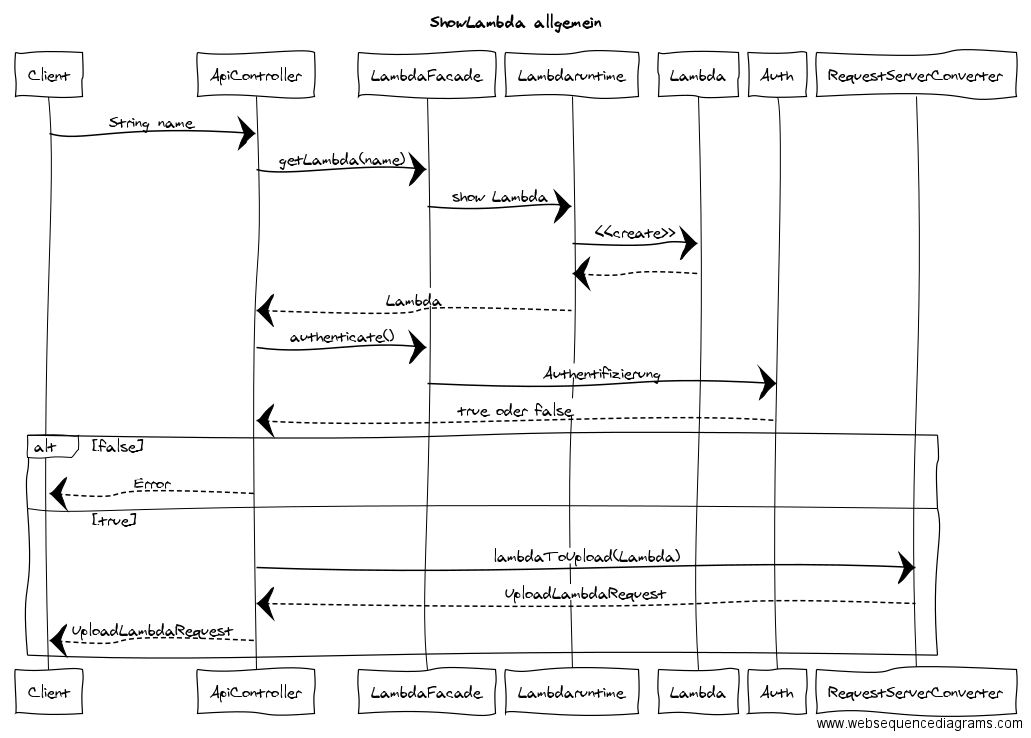
\includegraphics[width=18cm,height=12cm]{ShowLambda}
\end{figure}
\newpage
\subsection{Löschen}
	\begin{figure}[!hb]
    \includegraphics[width=18cm,height=19cm]{Delete}
\end{figure}
\newpage
	\section{Authentifizierung}
	\subsection{Spring Security Anbindung}	
	\begin{figure}[!hb]
    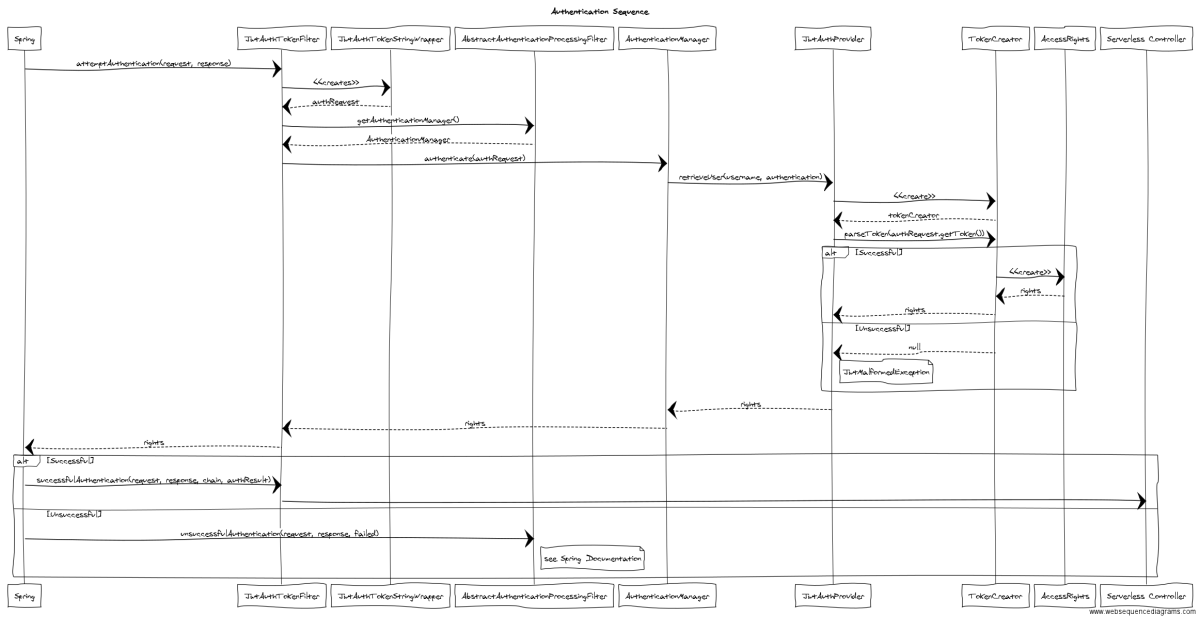
\includegraphics[width=18cm,height=12cm]{auth}
	\end{figure}
	\newpage
	\subsection{Runtime Anbindung}	
	\begin{figure}[!hb]
    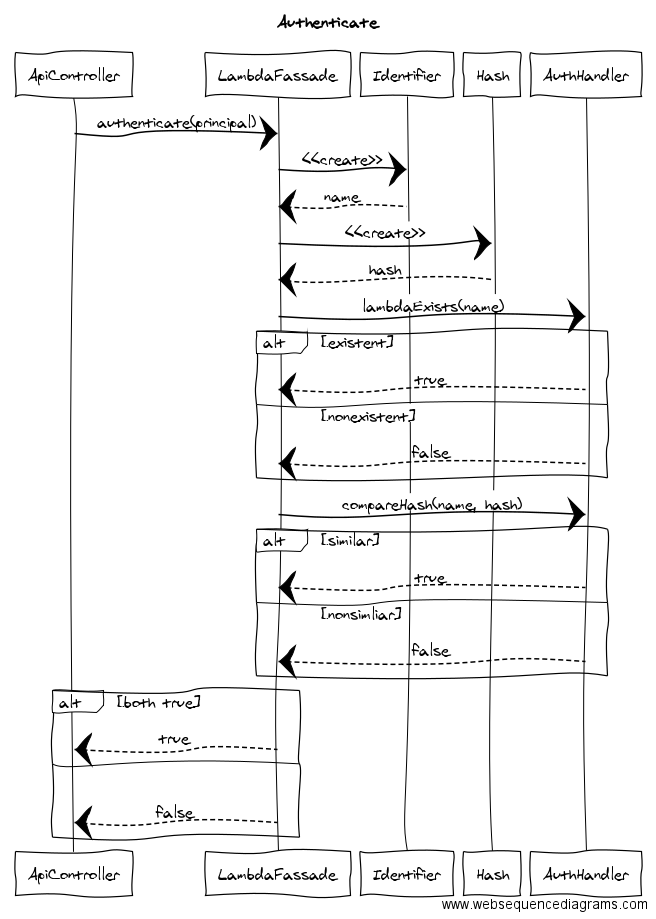
\includegraphics[width=18cm,height=18cm]{Authenticate}
	\end{figure}
	\newpage
	\subsection{Subtoken erstellen}
	\begin{figure}[!hb]
    \includegraphics[width=18cm,height=18cm]	{Subtoken}
	\end{figure}
	\newpage
	\section{Runtime}
	\subsection{Initialisierung}
	\begin{figure}[!hb]
    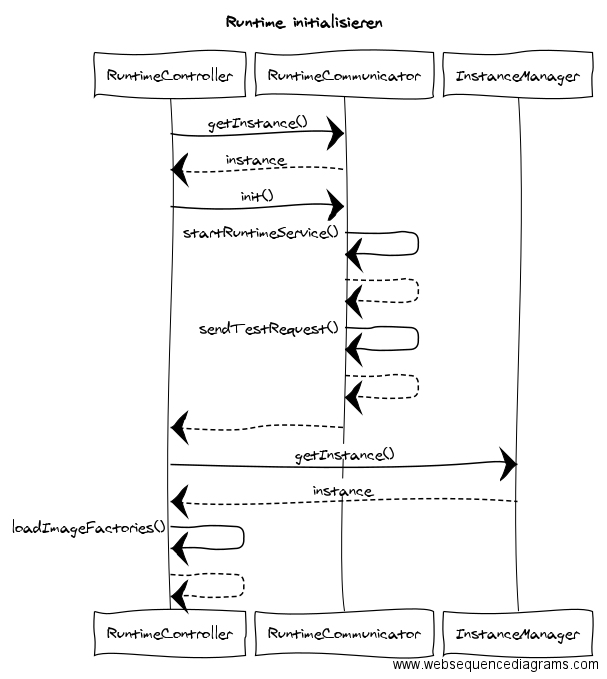
\includegraphics[width=18cm,height=16cm]{runtimeInit}
\end{figure}
\newpage
	\subsection{Image bauen}
	\begin{figure}[!hb]
    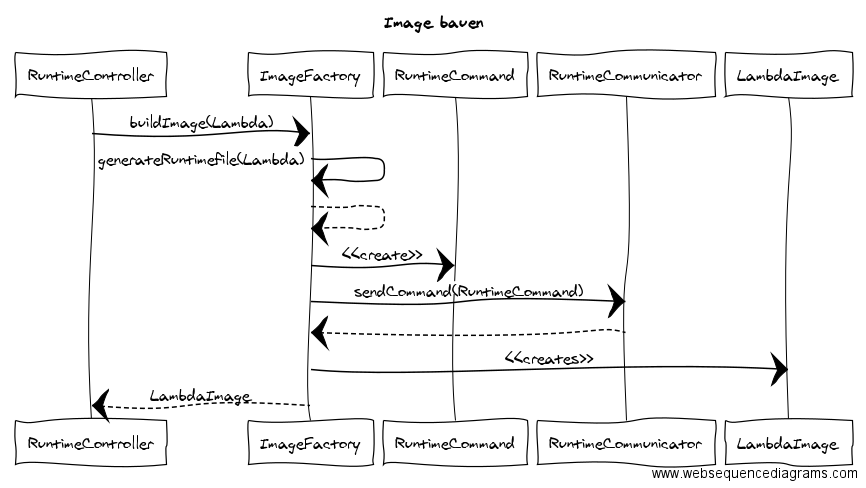
\includegraphics[width=18cm,height=15cm]{buildImage}
\end{figure}
\newpage
\subsection{Image umbauen}
	\begin{figure}[!hb]
    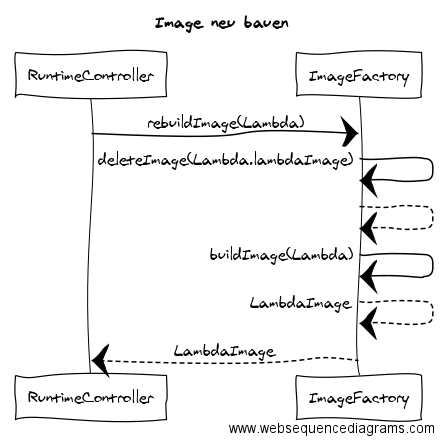
\includegraphics[width=18cm,height=16cm]{rebuildImage}
\end{figure}
\newpage
\subsection{Image löschen}
	\begin{figure}[!hb]
    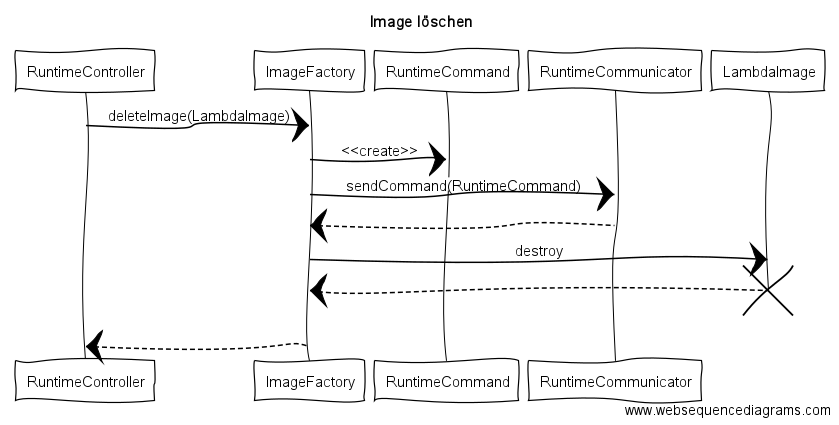
\includegraphics[width=18cm,height=13cm]{deleteImage}
\end{figure}
\newpage
\subsection{Image starten}
	\begin{figure}[!hb]
    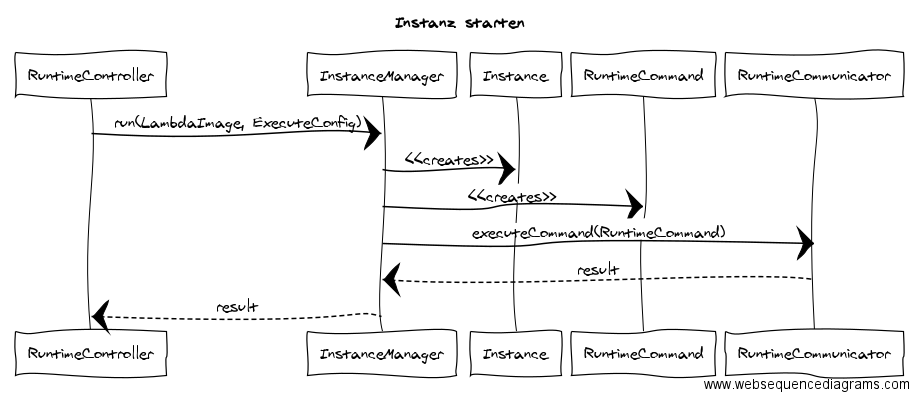
\includegraphics[width=18cm,height=13cm]{startInstance}
\end{figure}
\newpage
\newpage	
	
	\chapter{Dateiformate}
	In diesem Kapitel werden die Bedingungen für JSON-Dateien beschrieben, die der Benutzer für API-Befehle eingeben muss. Hier wird das Format des Parameters "config" beschrieben. Falls irgendeine Bedingung nicht erfüllt wird, bekommt der Nutzer sofort eine Fehlermeldung mit einer Beschreibung drüber, was falsch eingegeben wurde.

	\section{Hochladen/Anpassen von Lambda-Funktionen: Konfigurationsdatei}
	Diese \textbf{JSON}-Datei muss beim Nutzer eingegeben werden, um eine Funktion hochzuladen/zu ändern. Diese Datei beschreibt die Einstellungen einer  Funktion, die der Nutzer hochladen will. 
	\begin{lstlisting}
	{
	"name": <Name_of_Lambda>, 
	"language": <Language_of_Lambda>, 
	"parameters_input": [<type0>, <type1>], 
	"libraries":[library0, library1], 
	"code": <Code>
	}	
	\end{lstlisting}
	\begin{itemize}
		\item \textbf{name} - Name der Lambda-Funktion. Dieser Parameter muss dem folgenden regulären Ausdruck entsprechen: [A-Za-z\_]+[0-9]*, z.B. \textit{foo21, \_foo, Func12\_12}
		\item \textbf{language} - Programmiersprache der Lambda-Funktion, z.B. \textit{ Java, Python2, C\#}
		\item \textbf{parameters\_input} - Parametertypen der Eingaben der Lambda-Funktion, z.B. \textit{String, int, double[]} .
		\item \textbf{libraries} - Bibliotheken, die die Lambda-Funktion benutzt, z.B. \textit{math.h, swing, JavaUtil}
		\item \textbf{code} - Text der Lambda-Funktion, z.B. \textit{print("Hello Serverless");}
	\end{itemize}
	\clearpage
	\section{Ausführung von Lambda-Funktionen }
	Diese \textbf{JSON}-Datei muss beim Nutzer eingegeben werden, um eine Funktion auszuführen. Diese Datei beschreibt die Einstellungen für die Ausführung einer Funktion.
	\begin{lstlisting}
	{
	"times": <number_of_times_running>,
	"parameters_input":[<input0>,<input1>] 
	}
	\end{lstlisting}
	\begin{itemize}
		\item \textbf{times} - Anzahl von Ausführungen der Funktion, z.B. \textit{1, 3, 100}
		\item \textbf{parameters\_input} - Eingabe, die eine Funktion bei der Ausführung bearbeiten muss, z.B. \textit{1,2, true}. 
	\end{itemize}
    
    \section{Generierung von Tokens}
    Diese \textbf{JSON}-Datei muss beim Nutzer eingegeben werden, um einen Subtoken zu erstellen. Diese Datei beschreibt die Einstellungen für Tokengenerierung.
    \begin{lstlisting}
    {
      "expires": time
    }
    \end{lstlisting}
    \begin{itemize}
    	\item \textbf{expires} - Zeit in Minuten, die beschreibt wie lange ein Subtoken gültig sein wird, z.B. \textit{23}.
 
    \end{itemize}
    
    
	
		
	
	\printglossaries
\end{document}
